%% bare_jrnl.tex
%% V1.4b
%% 2015/08/26
%% by Michael Shell
%% see http://www.michaelshell.org/
%% for current contact information.
%%
%% This is a skeleton file demonstrating the use of IEEEtran.cls
%% (requires IEEEtran.cls version 1.8b or later) with an IEEE
%% journal paper.
%%
%% Support sites:
%% http://www.michaelshell.org/tex/ieeetran/
%% http://www.ctan.org/pkg/ieeetran
%% and
%% http://www.ieee.org/

%%*************************************************************************
%% Legal Notice:
%% This code is offered as-is without any warranty either expressed or
%% implied; without even the implied warranty of MERCHANTABILITY or
%% FITNESS FOR A PARTICULAR PURPOSE! 
%% User assumes all risk.
%% In no event shall the IEEE or any contributor to this code be liable for
%% any damages or losses, including, but not limited to, incidental,
%% consequential, or any other damages, resulting from the use or misuse
%% of any information contained here.
%%
%% All comments are the opinions of their respective authors and are not
%% necessarily endorsed by the IEEE.
%%
%% This work is distributed under the LaTeX Project Public License (LPPL)
%% ( http://www.latex-project.org/ ) version 1.3, and may be freely used,
%% distributed and modified. A copy of the LPPL, version 1.3, is included
%% in the base LaTeX documentation of all distributions of LaTeX released
%% 2003/12/01 or later.
%% Retain all contribution notices and credits.
%% ** Modified files should be clearly indicated as such, including  **
%% ** renaming them and changing author support contact information. **
%%*************************************************************************


% *** Authors should verify (and, if needed, correct) their LaTeX system  ***
% *** with the testflow diagnostic prior to trusting their LaTeX platform ***
% *** with production work. The IEEE's font choices and paper sizes can   ***
% *** trigger bugs that do not appear when using other class files.       ***                          ***
% The testflow support page is at:
% http://www.michaelshell.org/tex/testflow/



\documentclass[journal]{IEEEtran}
%
% If IEEEtran.cls has not been installed into the LaTeX system files,
% manually specify the path to it like:
% \documentclass[journal]{../sty/IEEEtran}


% support chinese
\usepackage{ctex}
\usepackage{graphicx}
\usepackage{multirow}
% Some very useful LaTeX packages include:
% (uncomment the ones you want to load)


% *** MISC UTILITY PACKAGES ***
%
%\usepackage{ifpdf}
% Heiko Oberdiek's ifpdf.sty is very useful if you need conditional
% compilation based on whether the output is pdf or dvi.
% usage:
% \ifpdf
%   % pdf code
% \else
%   % dvi code
% \fi
% The latest version of ifpdf.sty can be obtained from:
% http://www.ctan.org/pkg/ifpdf
% Also, note that IEEEtran.cls V1.7 and later provides a builtin
% \ifCLASSINFOpdf conditional that works the same way.
% When switching from latex to pdflatex and vice-versa, the compiler may
% have to be run twice to clear warning/error messages.






% *** CITATION PACKAGES ***
%
%\usepackage{cite}
% cite.sty was written by Donald Arseneau
% V1.6 and later of IEEEtran pre-defines the format of the cite.sty package
% \cite{} output to follow that of the IEEE. Loading the cite package will
% result in citation numbers being automatically sorted and properly
% "compressed/ranged". e.g., [1], [9], [2], [7], [5], [6] without using
% cite.sty will become [1], [2], [5]--[7], [9] using cite.sty. cite.sty's
% \cite will automatically add leading space, if needed. Use cite.sty's
% noadjust option (cite.sty V3.8 and later) if you want to turn this off
% such as if a citation ever needs to be enclosed in parenthesis.
% cite.sty is already installed on most LaTeX systems. Be sure and use
% version 5.0 (2009-03-20) and later if using hyperref.sty.
% The latest version can be obtained at:
% http://www.ctan.org/pkg/cite
% The documentation is contained in the cite.sty file itself.






% *** GRAPHICS RELATED PACKAGES ***
%
\ifCLASSINFOpdf
  % \usepackage[pdftex]{graphicx}
  % declare the path(s) where your graphic files are
  % \graphicspath{{../pdf/}{../jpeg/}}
  % and their extensions so you won't have to specify these with
  % every instance of \includegraphics
  % \DeclareGraphicsExtensions{.pdf,.jpeg,.png}
\else
  % or other class option (dvipsone, dvipdf, if not using dvips). graphicx
  % will default to the driver specified in the system graphics.cfg if no
  % driver is specified.
  % \usepackage[dvips]{graphicx}
  % declare the path(s) where your graphic files are
  % \graphicspath{{../eps/}}
  % and their extensions so you won't have to specify these with
  % every instance of \includegraphics
  % \DeclareGraphicsExtensions{.eps}
\fi
% graphicx was written by David Carlisle and Sebastian Rahtz. It is
% required if you want graphics, photos, etc. graphicx.sty is already
% installed on most LaTeX systems. The latest version and documentation
% can be obtained at: 
% http://www.ctan.org/pkg/graphicx
% Another good source of documentation is "Using Imported Graphics in
% LaTeX2e" by Keith Reckdahl which can be found at:
% http://www.ctan.org/pkg/epslatex
%
% latex, and pdflatex in dvi mode, support graphics in encapsulated
% postscript (.eps) format. pdflatex in pdf mode supports graphics
% in .pdf, .jpeg, .png and .mps (metapost) formats. Users should ensure
% that all non-photo figures use a vector format (.eps, .pdf, .mps) and
% not a bitmapped formats (.jpeg, .png). The IEEE frowns on bitmapped formats
% which can result in "jaggedy"/blurry rendering of lines and letters as
% well as large increases in file sizes.
%
% You can find documentation about the pdfTeX application at:
% http://www.tug.org/applications/pdftex





% *** MATH PACKAGES ***
%
%\usepackage{amsmath}
% A popular package from the American Mathematical Society that provides
% many useful and powerful commands for dealing with mathematics.
%
% Note that the amsmath package sets \interdisplaylinepenalty to 10000
% thus preventing page breaks from occurring within multiline equations. Use:
%\interdisplaylinepenalty=2500
% after loading amsmath to restore such page breaks as IEEEtran.cls normally
% does. amsmath.sty is already installed on most LaTeX systems. The latest
% version and documentation can be obtained at:
% http://www.ctan.org/pkg/amsmath





% *** SPECIALIZED LIST PACKAGES ***
%
%\usepackage{algorithmic}
% algorithmic.sty was written by Peter Williams and Rogerio Brito.
% This package provides an algorithmic environment fo describing algorithms.
% You can use the algorithmic environment in-text or within a figure
% environment to provide for a floating algorithm. Do NOT use the algorithm
% floating environment provided by algorithm.sty (by the same authors) or
% algorithm2e.sty (by Christophe Fiorio) as the IEEE does not use dedicated
% algorithm float types and packages that provide these will not provide
% correct IEEE style captions. The latest version and documentation of
% algorithmic.sty can be obtained at:
% http://www.ctan.org/pkg/algorithms
% Also of interest may be the (relatively newer and more customizable)
% algorithmicx.sty package by Szasz Janos:
% http://www.ctan.org/pkg/algorithmicx




% *** ALIGNMENT PACKAGES ***
%
%\usepackage{array}
% Frank Mittelbach's and David Carlisle's array.sty patches and improves
% the standard LaTeX2e array and tabular environments to provide better
% appearance and additional user controls. As the default LaTeX2e table
% generation code is lacking to the point of almost being broken with
% respect to the quality of the end results, all users are strongly
% advised to use an enhanced (at the very least that provided by array.sty)
% set of table tools. array.sty is already installed on most systems. The
% latest version and documentation can be obtained at:
% http://www.ctan.org/pkg/array


% IEEEtran contains the IEEEeqnarray family of commands that can be used to
% generate multiline equations as well as matrices, tables, etc., of high
% quality.




% *** SUBFIGURE PACKAGES ***
%\ifCLASSOPTIONcompsoc
%  \usepackage[caption=false,font=normalsize,labelfont=sf,textfont=sf]{subfig}
%\else
 % \usepackage[caption=false,font=footnotesize]{subfig}
%\fi
% subfig.sty, written by Steven Douglas Cochran, is the modern replacement
% for subfigure.sty, the latter of which is no longer maintained and is
% incompatible with some LaTeX packages including fixltx2e. However,
% subfig.sty requires and automatically loads Axel Sommerfeldt's caption.sty
% which will override IEEEtran.cls' handling of captions and this will result
% in non-IEEE style figure/table captions. To prevent this problem, be sure
% and invoke subfig.sty's "caption=false" package option (available since
% subfig.sty version 1.3, 2005/06/28) as this is will preserve IEEEtran.cls
% handling of captions.
% Note that the Computer Society format requires a larger sans serif font
% than the serif footnote size font used in traditional IEEE formatting
% and thus the need to invoke different subfig.sty package options depending
% on whether compsoc mode has been enabled.
%
% The latest version and documentation of subfig.sty can be obtained at:
% http://www.ctan.org/pkg/subfig




% *** FLOAT PACKAGES ***
%
%\usepackage{fixltx2e}
% fixltx2e, the successor to the earlier fix2col.sty, was written by
% Frank Mittelbach and David Carlisle. This package corrects a few problems
% in the LaTeX2e kernel, the most notable of which is that in current
% LaTeX2e releases, the ordering of single and double column floats is not
% guaranteed to be preserved. Thus, an unpatched LaTeX2e can allow a
% single column figure to be placed prior to an earlier double column
% figure.
% Be aware that LaTeX2e kernels dated 2015 and later have fixltx2e.sty's
% corrections already built into the system in which case a warning will
% be issued if an attempt is made to load fixltx2e.sty as it is no longer
% needed.
% The latest version and documentation can be found at:
% http://www.ctan.org/pkg/fixltx2e


%\usepackage{stfloats}
% stfloats.sty was written by Sigitas Tolusis. This package gives LaTeX2e
% the ability to do double column floats at the bottom of the page as well
% as the top. (e.g., "\begin{figure*}[!b]" is not normally possible in
% LaTeX2e). It also provides a command:
%\fnbelowfloat
% to enable the placement of footnotes below bottom floats (the standard
% LaTeX2e kernel puts them above bottom floats). This is an invasive package
% which rewrites many portions of the LaTeX2e float routines. It may not work
% with other packages that modify the LaTeX2e float routines. The latest
% version and documentation can be obtained at:
% http://www.ctan.org/pkg/stfloats
% Do not use the stfloats baselinefloat ability as the IEEE does not allow
% \baselineskip to stretch. Authors submitting work to the IEEE should note
% that the IEEE rarely uses double column equations and that authors should try
% to avoid such use. Do not be tempted to use the cuted.sty or midfloat.sty
% packages (also by Sigitas Tolusis) as the IEEE does not format its papers in
% such ways.
% Do not attempt to use stfloats with fixltx2e as they are incompatible.
% Instead, use Morten Hogholm'a dblfloatfix which combines the features
% of both fixltx2e and stfloats:
%
% \usepackage{dblfloatfix}
% The latest version can be found at:
% http://www.ctan.org/pkg/dblfloatfix




%\ifCLASSOPTIONcaptionsoff
%  \usepackage[nomarkers]{endfloat}
% \let\MYoriglatexcaption\caption
% \renewcommand{\caption}[2][\relax]{\MYoriglatexcaption[#2]{#2}}
%\fi
% endfloat.sty was written by James Darrell McCauley, Jeff Goldberg and 
% Axel Sommerfeldt. This package may be useful when used in conjunction with 
% IEEEtran.cls'  captionsoff option. Some IEEE journals/societies require that
% submissions have lists of figures/tables at the end of the paper and that
% figures/tables without any captions are placed on a page by themselves at
% the end of the document. If needed, the draftcls IEEEtran class option or
% \CLASSINPUTbaselinestretch interface can be used to increase the line
% spacing as well. Be sure and use the nomarkers option of endfloat to
% prevent endfloat from "marking" where the figures would have been placed
% in the text. The two hack lines of code above are a slight modification of
% that suggested by in the endfloat docs (section 8.4.1) to ensure that
% the full captions always appear in the list of figures/tables - even if
% the user used the short optional argument of \caption[]{}.
% IEEE papers do not typically make use of \caption[]'s optional argument,
% so this should not be an issue. A similar trick can be used to disable
% captions of packages such as subfig.sty that lack options to turn off
% the subcaptions:
% For subfig.sty:
% \let\MYorigsubfloat\subfloat
% \renewcommand{\subfloat}[2][\relax]{\MYorigsubfloat[]{#2}}
% However, the above trick will not work if both optional arguments of
% the \subfloat command are used. Furthermore, there needs to be a
% description of each subfigure *somewhere* and endfloat does not add
% subfigure captions to its list of figures. Thus, the best approach is to
% avoid the use of subfigure captions (many IEEE journals avoid them anyway)
% and instead reference/explain all the subfigures within the main caption.
% The latest version of endfloat.sty and its documentation can obtained at:
% http://www.ctan.org/pkg/endfloat
%
% The IEEEtran \ifCLASSOPTIONcaptionsoff conditional can also be used
% later in the document, say, to conditionally put the References on a 
% page by themselves.




% *** PDF, URL AND HYPERLINK PACKAGES ***
%
%\usepackage{url}
% url.sty was written by Donald Arseneau. It provides better support for
% handling and breaking URLs. url.sty is already installed on most LaTeX
% systems. The latest version and documentation can be obtained at:
% http://www.ctan.org/pkg/url
% Basically, \url{my_url_here}.




% *** Do not adjust lengths that control margins, column widths, etc. ***
% *** Do not use packages that alter fonts (such as pslatex).         ***
% There should be no need to do such things with IEEEtran.cls V1.6 and later.
% (Unless specifically asked to do so by the journal or conference you plan
% to submit to, of course. )


% correct bad hyphenation here
\hyphenation{op-tical net-works semi-conduc-tor}


\begin{document}
%
% paper title
% Titles are generally capitalized except for words such as a, an, and, as,
% at, but, by, for, in, nor, of, on, or, the, to and up, which are usually
% not capitalized unless they are the first or last word of the title.
% Linebreaks \\ can be used within to get better formatting as desired.
% Do not put math or special symbols in the title.
\title{寻找一种易于理解的一致性算法\\(扩展版)}
%
%
% author names and IEEE memberships
% note positions of commas and nonbreaking spaces ( ~ ) LaTeX will not break
% a structure at a ~ so this keeps an author's name from being broken across
% two lines.
% use \thanks{} to gain access to the first footnote area
% a separate \thanks must be used for each paragraph as LaTeX2e's \thanks
% was not built to handle multiple paragraphs
%

\author{Diego Ongaro and John Ousterhout \\ Stanford University}

% note the % following the last \IEEEmembership and also \thanks - 
% these prevent an unwanted space from occurring between the last author name
% and the end of the author line. i.e., if you had this:
% 
% \author{....lastname \thanks{...} \thanks{...} }
%                     ^------------^------------^----Do not want these spaces!
%
% a space would be appended to the last name and could cause every name on that
% line to be shifted left slightly. This is one of those "LaTeX things". For
% instance, "\textbf{A} \textbf{B}" will typeset as "A B" not "AB". To get
% "AB" then you have to do: "\textbf{A}\textbf{B}"
% \thanks is no different in this regard, so shield the last } of each \thanks
% that ends a line with a % and do not let a space in before the next \thanks.
% Spaces after \IEEEmembership other than the last one are OK (and needed) as
% you are supposed to have spaces between the names. For what it is worth,
% this is a minor point as most people would not even notice if the said evil
% space somehow managed to creep in.



% The paper headers
 \markboth{T\MakeLowercase{ranslated by} L\MakeLowercase{inqiang} W\MakeLowercase{ang} \MakeLowercase{(https://github.com/brandonwang001/raft\_translation)}}%
 {Shell \MakeLowercase{\textit{et al.}}: Bare Demo of IEEEtran.cls for IEEE Journals}
% The only time the second header will appear is for the odd numbered pages
% after the title page when using the twoside option.
% 
% *** Note that you probably will NOT want to include the author's ***
% *** name in the headers of peer review papers.                   ***
% You can use \ifCLASSOPTIONpeerreview for conditional compilation here if
% you desire.




% If you want to put a publisher's ID mark on the page you can do it like
% this:
% \IEEEpubid{0000--0000/00\$00.00~\copyright~2015 IEEE}
% Remember, if you use this you must call \IEEEpubidadjcol in the second
% column for its text to clear the IEEEpubid mark.



% use for special paper notices
%\IEEEspecialpapernotice{(Invited Paper)}




% make the title area
\maketitle

% As a general rule, do not put math, special symbols or citations
% in the abstract or keywords.
\begin{abstract}
Raft是一种基于日志复制的一致性算法。Raft的结果等价于(multi-)Paxos并且和Paxos一样的有效,但却和Paxos的结构完全不同。正是Raft不同于Paxos的结构使得Raft更容易理解,并且更易于工程实现。Raft通过将一致性关键点进行拆解,包含选主、日志复制和安全三部分,另外通过减少状态机的状态使得Raft更容易理解。通过学生学习Raft和Paxos的分析,结果显示Raft相比于Paxos更容易理解。Raft创新的使用了一种新的机制来处理集群中机器的变更。
\end{abstract}

% Note that keywords are not normally used for peerreview papers.
% \begin{IEEEkeywords}
% EEE, IEEEtran, journal, \LaTeX, paper, template.
% \end{IEEEkeywords}






% For peer review papers, you can put extra information on the cover
% page as needed:
% \ifCLASSOPTIONpeerreview
% \begin{center} \bfseries EDICS Category: 3-BBND \end{center}
% \fi
%
% For peerreview papers, this IEEEtran command inserts a page break and
% creates the second title. It will be ignored for other modes.
\IEEEpeerreviewmaketitle



\section{简介}
% The very first letter is a 2 line initial drop letter followed
% by the rest of the first word in caps.
% 
% form to use if the first word consists of a single letter:
% \IEEEPARstart{A}{demo} file is ....
% 
% form to use if you need the single drop letter followed by
% normal text (unknown if ever used by the IEEE):
% \IEEEPARstart{A}{}demo file is ....
% 
% Some journals put the first two words in caps:
% \IEEEPARstart{T}{his demo} file is ....
% 
% Here we have the typical use of a "T" for an initial drop letter
% and "HIS" in caps to complete the first word.
一致性算法可以使得若干机器像一个一致集群一样的工作,即使在集群成员变更或者宕机的情况下,整个集群仍然可以正常工作。正因为如此一致性算法在大规模分布式系统中扮演着至关重要的角色。过去的十年,paxos统治了整个一致性算法。大多数一致性算法的实现都是基于Paxos或者受到Paxos的影响,同时一致性算法课程大多也是讲授Paxos。


不幸的是,Paxos晦涩难懂,尽管很多人努力尝试让Paxos更容易理解。除此之外,在实际系统中,实现者必须根据系统作出大量的调整。结果,系统开发者和学生都为了理解Paxos在苦苦挣扎。


我们也是苦苦的与Paxos斗争,后来我们希望找到一个既容易实现又利于学生学习的一致性算法。所以我们寻找一致性算法的首要目标就是易于理解:我们可以定义一种比Paxos利于实现和学习的一致性算法?进一步我们希望算法可以让系统开发者有直观感受和理解。我们认为算法能工作很重要,更重要的是让算法实现者直观到理解它为什么可以工作。


为了设计Raft算法,我们使用了特定的技术来使算法更容易理解,包括分解法(Raft分解为选主、日志复制和安全)和状态空间简化(相较于Paxos,Raft减少了未定状态的数量)。我们分析两个学校43名同学的学习情况,结果显示Raft比Paxos更容易理解:学习过两种算法后,他们中的33位同学可以更好的解答Raft中的问题相比于Paxos。


Raft和存在的一些一致性算法是相似的,但是也有它自己新颖的特点:
\begin{itemize}
\item \textbf{Strong leader:}Raft使用了一种比其它一致性算法更强的leader。比如,日志记录只能从leader复制到其它机器,这样可以简化日志复制和降低理解难度。
\item \textbf{Leader election:}Raft使用了随机定时器来选择leader。通过在心跳上增加一些小的改动,可以简单快速的解决冲突。
\item \textbf{Membership changes:}Raft使用了一种联合一致性的方法,使得集群中的机器发生变更的时候,整个集群也可以正常的工作。联合一致性配置是两个不同配置的大多数机器的重叠。
\end{itemize}


我们相信Raft不管是在教学或者实现方面都是优于其它一致性算法。我们详细的描述可以让开发者更简单的进行系统的实现。另外已经有几个公司公开了自己的实现,Raft的安全性是验证和证明的,同样它也和其它一致性算法一样有效。


文章接下来会在第二节讲述复制状态机,第三节会讨论Paxos的优缺点,第四节会描述易于理解方法,第五-八节会描述Raft一致性算法,第九节会评估Raft,第十节讨论我们的相关工作。

\section{复制状态机}
通常提到一致性算法都会提到复制状态机[37]。在复制状态机中,集群中所有的机器有相同的日志副本,即使集群中某些集群宕机,整个集群仍然可以正常工作。复制状态机通常被用来解决分布式系统的容错问题。
\begin{figure}[htbp]
\begin{center}
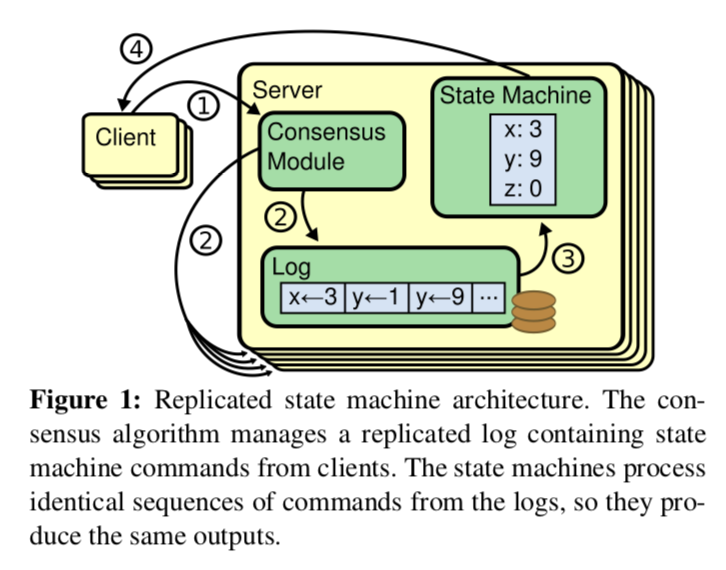
\includegraphics[width=1\linewidth]{./fig1.png}
%\caption{default}
%\label{default}
\end{center}
\end{figure}
例如:例如GFS、HDFS和RAMCloud等大规模系统中,通常使用分离的状态机来管理选主和存储配置信息。Chubby和ZooKeeper中也使用了复制状态机。


复制状态机通常是通过复制日志来实现的,如图1所示。每个机器的log文件中包含了一系列的命令,这些命令将会被按顺序执行到状态机。每个机器的日志包含相同的命令并且命令都有相同的顺序,如果状态机按相同的顺序执行命令。由于状态机初始化状态是相同的,并且按照相同顺序执行相同的命令,那么必然状态机有相同的输出。


一致性算法的工作就是保证各个状态机一致。机器上的一致性模块接受到来自客户端的命令,并把命令追加到自己的日志中。然后和其它机器上的一致性模块进行通信来保证最终所有机器都按相同的顺序存储了请求,即使其中的一些机器宕机不能工作。一旦命令被正确的复制,每个机器都按照日志顺序将命令执行到状态机,然后将输出返回给客户端。最终,所有的机器呈现一个高度可靠的状态机。

实际系统的一致性算法具有一下的特性:
\begin{itemize}
\item 在非拜占庭条件下必须是安全的,不会返回错误的结果。例如:网络延时、分区、丢包、重复和乱序等。
\item 在集群中大多数机器可以正常工作的情况下,整个集群必须是可用的。一个5机器的集群可以容忍两台机器的宕机。我们假定机器宕机后可以从稳定存储介质恢复并重新加入到集群中。
\item 它们不依赖时间来保证日志的的一致性:错误的时钟和巨大的消息延迟,在极端情况下,会导致集群的不可用。
\item 在正常情况下,集群中的机器在一轮RPC下就可以完成一次日志的复制,个别较慢的机器不能影响整个系统的性能。
\end{itemize}

\section{Paxos存在的问题}
过去十年,Leslie Lamport的Paxos算法等同于一致性算法。许多学校会教授Paxos算法,许多算法也是依据Paxos进行实现的。Paxos是第一个能对单次提议达成一致的协议,就好像单条日志复制。我们把达成单次一致的协议称为\textit{single-decree Paxos}。Paxos通过一系列单次一致的实例来达到对一系列的提议达成一致,这被称作\textit{multi-Paxos}。Paxos算法可以保证安全和存活,同时也支持集群成员变更。Paxos的正确性是被证明的,并且在正常情况下是有效的。


不幸的是,Paxos有个显著的缺点。第一个缺点就是Paxos晦涩难懂。很多人投入大量的经历,但是只有很少的人真正的理解Paxos。已经有很多学者尝试以更容易理解的方式解释Paxos。这些解释都是集中在\textit{single-decree Paxos},但是仍然存在很大的挑战。通过调研我们发现很多人不满Paxos,即使很多很有经验的研究者。为了设计我们的算法,我们阅读了很多简单的解释,并尝试设计可用的算法,整个过程花费大约1年的时间。


我们认为Paxis晦涩难懂的原因是因为Paxos选择了\textit{single-decree Paxos}作为基本的子问题导致的。\textit{single-decree Paxos}是紧凑且精巧的,它的两个阶段是不能独立分开的,并且通过简单的直觉进行理解和解释。正因为如此,很难形成\textit{single-decree Paxos}为什么可以正常工作的直觉。\textit{multi-Paxos}更是增加了额外的复杂度和精密度。我们相信整个问题可以达到一致是通过多次的决定,并且可以被拆分进行直观的理解。


Paxos存在第二个问题是它不能简单的转化为工程实现,一方面是大家没有对\textit{multi-Paxos}算法达成一致。Lamport大神只是详细的描述了\textit{single-decree Paxos},但是很多细节还是缺失的。还存在很多基于Paxos的变种和分支。Chubby是基于Paxos进行实现的,但是它们的实现细节并没有公开。


另外,Paxos的结构决定它很难用来实现实际的系统,这是\textit{single-decree Paxos}不能分解导致的必然结果。举个例子,通过单独的选择日志记录的集合并把它们聚合在一个顺序日志中,并不能带来太多的收益,但是却增加了额外的复杂度。设计一种只是按照严格顺序进行追加的日志是简单和更为有效的。此外Paxos采用了对称的点对点通信的方法作为它的核心(尽管是出于一种基于弱领导的性能优化)。上面的优化仅仅对于单次决定是有意义的,但是实际系统很少采用这种方法。如果有一些的提议需要被决定,首先选举出一个leader然后由leader进行协调,这样是更为简单和快速的。


现实中的系统仅有很少和Paxos中描述的系统相似。每个实际系统都是从Paxos开始,发现实现中有很多不能解决的难题,然后提出一个新的结构并实现。这是耗时且容易犯错的,然后Paxos的晦涩难懂进一步使情况恶化。Paxos的范式可能是一种证明一致性理论的好方法,但是实际的实现中Paxos不具备很大的价值。下面来自Chubby开发者的评论更正说明这一点:


\textit{实际系统的实现和Paxos所描述的算法中存在巨大的鸿沟...最终实现的系统将是基于一个未被证明的协议}


因为这些问题的存在,我们认为Paxos并不适合系统实现和教学。在大规模软件系统中一致性至关重要,我们决定尝试是否可以设计一种和Paxos有相同特性且易于理解的算法。Raft正是我们试验的产物。




\section{为了理解而设计}
设计Raft时,我们有几个目标:它对于系统的开发必须是完整和易于实现的,这样可以减少开发者大量不必要的设计工作;它必须在所有条件下是安全的,并在典型条件下是可用的;另外对于正常操作它必须是有效的。但我们最重要的目标是(也是最大的挑战)是易理解性。它必须是大多数读者可以舒适的理解的。此外,它必须可以让系统开发者有直观的感受,这样系统开发者可以在实际的实现中可以更好的进行扩展。

下面会列举一些在设计Raft算法过程中,怎样从很多候选的方法中进行选择的考虑点。我们还是根据候选方法的可理解性来进行评估:每种候选的方法是否易于解释的?(例如,它的状态机空间复杂?它是否有暗含的精巧设计?)是不是可以让一个读者很容易的理解它的潜在表达。


我们承认这样的分析存在很大主观成分,不可否认的是我们使用了两种通用的技术:第一个技术是众所周知的问题分解法,我们尽可能将问题分解为独立的可以被解决,易于解释和理解的子问题。例如:在Raft中我们利用问题分解法分为4个独立的问题:选主、日志复制、安全和成员变更。


第二个技术是通过减少需要考虑的状态来简化状态空间。这样使得系统更加一致并尽可能消除不确定的状态。特别的,Raft不允许日志中出现空洞,并且禁止这样的情况发生。空洞会导致集群中的日志产生不一致。尽管我们尽力来消除不确定状态,但是在一些情况下,增加不确定状态可以更好的帮助理解算法。特别是,随机化方法会引进不确定状态,但是它可以简化状态空间通过以相同的方式来处理所有可能的选择("choose any; it doesnt matter")。我们使用了随机化的方法来简化Raft的选主算法。


\section{Raft一致性算法}
Raft是一种管理如第二节所描述的状态机的算法。图2以紧凑的格式总结了算法中的术语和定义。图3列举了算法的关键特性;这些图中的定义和术语将会在接下来的章节进行详细的讲解。


Raft实现一致性是首先选择一个确定的leader,然后leader负责管理日志复制。leader接受来自客户端的请求并追加到本地日志,然后把日志复制到其它的机器并告诉其它机器什么时候可以安全的将日志应用到状态机。集群存在一个leader的好处可以简化日志复制的管理。例如,leader可以决定日志的追加,而不需要经其它机器的同意。整个集群的数据流向也是从leader流向其它机器。如果leader宕机或者网络断开,其它的机器可以重新选举一个新的leader。


使用选主的方法,Raft可以将一致性问题分解为3个相对独立的子问题,下面的子章节将对这些问题进行讨论:

\begin{itemize}
\item \textbf{Leader election:}第5.2节将讨论,当一个leader宕机后,一个新的leader必须被选举。
\item \textbf{Log replication:}leader必须响应客户端的请求,并把日志复制到整个集群来保证其它机器的日志和自己的相同。
\item \textbf{Safety:}图3中的状态机的安全是Raft优先保证的:如果任意一台机器将一条特定的日志应用到自己的状态机,那么其他的机器就不能应用一条不同的日志到自己的状态机。在5.4节描述了Raft是如何保证这个特性的;解决这个问题的方案就是在选举是增加额外的规则约束(5.2节)。
\end{itemize}


在讲述完一致性算法后,这一章节还会讨论可用性的问题和时间在系统中的角色。

\begin{table}[htp]
\begin{center}
\begin{tabular}{|p{2cm}p{6cm}|}
\hline
\multicolumn{2}{|c|}{\textbf{State}}  \\
\hline
\multicolumn{2}{|l|}{\textbf{所有机器需要持久化的状态:}} \\
\multicolumn{2}{|l|}{(在RPC响应之前,需要更新稳定存储介质)} \\
&\\
\textbf{currentTerm} & server存储的最新任期(初始化为0且单调递增)\\
&\\
\textbf{votedFor} & 当前任期接受到的选票的候选者ID(初值为null)\\
&\\
\textbf{log[]} & 日志记录 每条日记记录包含状态机的命令 \\ 
&\\
 & 和从leader接受到日志的任期。(索引初始化为1) \\
&\\
\multicolumn{2}{|l|}{\textbf{所有机器的可变状态:}} \\
\textbf{commitIndex} & 将被提交的日志记录的索引(初值为0且单调递增)\\
&\\
\textbf{lastApplied} & 已经被提交到状态机的最后一个日志的索引(初值为0且单调递增)\\
&\\
\multicolumn{2}{|l|}{\textbf{leader的可变状态:}} \\
\multicolumn{2}{|l|}{(每次选举后重新初始化)} \\
&\\
\textbf{nextIndex[]} & 每台机器在数组占据一个元素,元素的值为下条发送到该机器的日志索引 (初始值为leader最新一条日志的索引+1)\\
&\\
\textbf{matchIndex[]} & 每台机器在数组中占据一个元素,元素的记录将要复制给该机器日志的索引的。\\
\hline
\end{tabular}
\end{center}
\label{default}
\end{table}%

\begin{table}[htp]
\begin{center}
\begin{tabular}{|p{2cm}p{6cm}|}
\hline
\multicolumn{2}{|c|}{\textbf{AppendEntries RPC}}  \\
\hline
\multicolumn{2}{|l|}{\textbf{被leader用来复制日志(5.3节);同时也被用作心跳(5.2节)}} \\
&\\
\multicolumn{2}{|l|}{\textbf{Arguments:}} \\
&\\
\textbf{term} & leader任期\\
\textbf{leaderId} & 用来follower重定向到leader\\
\textbf{prevLogIndex} & 前继日志记录的索引 \\ 
\textbf{prevLogItem} & 前继日志的任期 \\
\textbf{entries[]} & 存储日志记录\\
\textbf{leaderCommit} & leader的commitIndex\\
&\\
\multicolumn{2}{|l|}{\textbf{Results:}} \\
\textbf{term} & 当前任期,leader用来更新自己\\
\textbf{success} & 如果follower包含索引为prevLogIndex和任期为prevLogItem的日志\\
&\\
\multicolumn{2}{|l|}{\textbf{接受者的实现:}} \\
\multicolumn{2}{|l|}{1. 如果leader的任期小于自己的任期返回false。(5.1)} \\
\multicolumn{2}{|l|}{2. 如果自己不存在索引、任期和prevLogIndex、prevLogItem} \\
\multicolumn{2}{|l|}{\ \ \ 匹配的日志返回false。(5.3)}\\
\multicolumn{2}{|l|}{3. 如果存在一条日志索引和prevLogIndex相等,}\\
\multicolumn{2}{|l|}{\ \ \ 但是任期和prevLogItem不相同的日志,}\\
\multicolumn{2}{|l|}{\ \ \ 需要删除这条日志及所有后继日志。(5.3)}\\
\multicolumn{2}{|l|}{4. 如果leader复制的日志本地没有,则直接追加存储。}\\
\multicolumn{2}{|l|}{5. 如果leaderCommit>commitIndex,}\\
\multicolumn{2}{|l|}{\ \ \ 设置本地commitIndex为leaderCommit和最新日志索引中}\\
\multicolumn{2}{|l|}{\ \ \ 较小的一个。}\\
\hline
\end{tabular}
\end{center}
\label{default}
\end{table}%



\begin{table}[htp]
\begin{center}
\begin{tabular}{|p{2cm}p{6cm}|}
\hline
\multicolumn{2}{|c|}{\textbf{RequestVote RPC}}  \\
\hline
\multicolumn{2}{|l|}{\textbf{被候选者用来收集选票:}} \\
&\\
\multicolumn{2}{|l|}{\textbf{Arguments:}} \\
&\\
\textbf{term} & 候选者的任期\\
\textbf{candidateId} & 候选者编号\\
\textbf{lastLogIndex} & 候选者最后一条日志记录的索引 \\ 
\textbf{lastLogItem} & 候选者最后一条日志记录的索引的任期 \\
&\\
\multicolumn{2}{|l|}{\textbf{Results:}} \\
\textbf{term} & 当前任期,候选者用来更新自己\\
\textbf{voteGranted} & 如果候选者当选则为true。\\
&\\
\multicolumn{2}{|l|}{\textbf{接受者的实现:}} \\
\multicolumn{2}{|l|}{1. 如果leader的任期小于自己的任期返回false。(5.1)} \\
\multicolumn{2}{|l|}{2. 如果本地voteFor为空,候选者日志和本地日志相同,} \\
\multicolumn{2}{|l|}{\ \ \ 则投票给该候选者(5.2和5.4)}\\
\hline
\end{tabular}
\end{center}
\label{default}
\end{table}%


\begin{table}[htp]
\begin{center}
\begin{tabular}{|p{8.4cm}|}
\hline
\textbf{Rules for Servers}  \\
\hline
\textbf{所有机器:} \\
1. 如果commitIndex > lastApplied:增加lastApplied,并将日志 \\
\ \ \ log[lastApplied]应用到状态机。 \\
2. 如果RPC请求中或者响应中包含任期T>currentTerm,\\
\ \ 参与者\ 该机器转化为参与者。\\
\\
\textbf{参与者(5.2节):}\\
1. 响应来自候选者或者leader的请求。\\
2. 如果选举定时器超时时,没有收到leader的的追加日志请求\\
\ \ \ 或者没有投票给候选者,该机器转化为候选者。\\
\\
\textbf{候选者(5.2节):}\\
1. 一旦变为候选者,则开始启动选举:\\
\ \ \ 1.1 增加currentTerm \\
\ \ \ 1.2 选举自己 \\
\ \ \ 1.3 重置选举定时器 \\
\ \ \ 1.4 并行发送选举请求到其他所有机器 \\
2. 如果收到集群大多数机器的选票,则称为新的leader。\\
3. 如果接受到新leader的追加日志请求,则转化为参与者。 \\
4. 如果选举定时器超时,则重启选举。\\
\\
\textbf{leaders:}\\
1. 一旦当选:发送空的追加日志请求(心跳)到其它所有机器;\\
\ \ \ 在空闲时间发送心跳,阻止其它机器的选举定时器超时。\\
2. 如果接受到来自客户端的请求,追加日志记录到本地日志,\\
\ \ \ 如果成功应用日志记录到状态机则回应客户端。\\
3. 如果某个参与者的最新日志索引大于等于本地存储该参与者的 \\ 
\ \ \ 最新日志索引:给该参与者发送包含从nextIndex开始的 \\
\ \ \ 日志追加请求。\\
\ \ \ 3.1 如果成功,更新该参与者的nextIndex和matchIndex。(5.3节)\\
\ \ \ 3.2 如果由于日志不一致而失败,减少nextIndex并重试。(5.3节) \\
4. 如果存在N > commitIndex(本地待提交日志的索引),\\
\ \ \ \ majority(matchIndex[i]>= N)(如果参与者大多数的\\
\ \ \ 最新日志的索引大于N), 并且这些参与者索引为N \\
\ \ \ 的日志的任期也等于leader的当前任期:commitIndex =N\\
\ \ \ (leader的待提交的日志索引设置为N)(5.2和5.4节)。\\
\hline
\end{tabular}
\end{center}
\label{default}
\end{table}%

\begin{table}[htp]
\begin{center}
\begin{tabular}{|p{8.4cm}|}
\hline
\\
\textbf{Election Safty:} 在一个给定的任期最多只可以选举出\\
\ \ \ 一个leader(5.2节)。\\
\textbf{Leader Append-Only:} 对于一个leader它永远不会重写和 \\ 
\ \ \ 删除日志中的日志记录,它只会追加日志记录。(5.3节)\\
\textbf{Log Matching:}如果两个日志文件中存在相同索引和任期的日志记录\\
\ \ \ 那么两个日志文件所有的日志记录在给定索引情况下\\
\ \ \ 是相同的。(5.3节)\\
\textbf{Leader Completeness:}如果一条日志在一个给定的任期已经提交,\\
\ \ \ 那么这条日志将会出现在所有任期大于给定任期的leader\\
\ \ \ 的日志中。(5.4节)\\
\textbf{State Machine Safety:}如果一个server已经将给定索引的日志\\
\ \ \ 应用到状态机,别的server将不能应用一个相同索引但内容不同的\\
\ \ \ 日志记录到自己的状态机。(5.4.3节)\\
\\
\hline
\multicolumn{1}{l}{}\\
\multicolumn{1}{l}{\textbf{Figure 3:} Raft guarantees that each of these properties is true}\\
\multicolumn{1}{l}{\qquad at all times. The section numbers indicate where each prop- }\\
\multicolumn{1}{l}{\qquad erty is discussed.}\\
\end{tabular}
\end{center}
\label{default}
\end{table}%


\subsection{Raft 基础}
一个Raft集群一般包含多台机器,5台机器是一种典型配置。它可以容忍集群中的两台机器不能正常工作。任意时刻,一台server会处在三种状态中的一种:leader、follower和candidate。正常情况下,集群中包含一个leader和参与者。集群中的参与者是被动的,它们不会主动解决问题而是被动的响应leader或者参与者的请求。集群中leader负责处理所有的客户端请求,如果一个客户端的请求连接到了参与者,这个参与者会将请求重定向到leader。候选者是在选举中可能成为leader的状态,如5.2节所描述。图4展示了这些状态,并描述了这些状态的迁移。


如图5所示,Raft将时间分为任意长度的间隔,每个间隔是一个任期。每个任期会由一个连续的整数进行表示。每个任期都是从选举开始的,在这个阶段会有一个或者多个候选者参与竞选,如图5所示。一旦某个候选者在选举中胜出,这个任期剩下的时间将有这个候选者作为leader。一些特殊的情况下,一次选举可能出现选举分裂的情况。选举分裂的情况下,当前任期将不会选举出leader。紧接着一个新的任期将会启动重新进行选举。Raft通过上面的过程保证每个任期只会选举出至多一个leader。

\begin{figure}[htbp]
\begin{center}
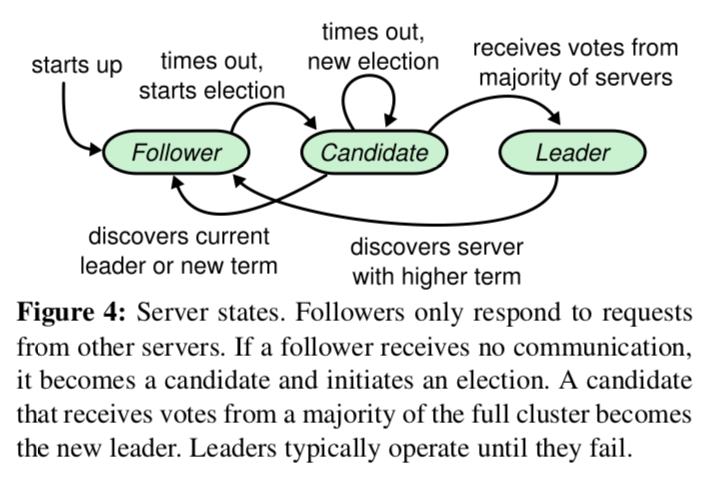
\includegraphics[width=1\linewidth]{./fig4.png}
%\caption{default}
%\label{default}
\end{center}
\end{figure}

\begin{figure}[htbp]
\begin{center}
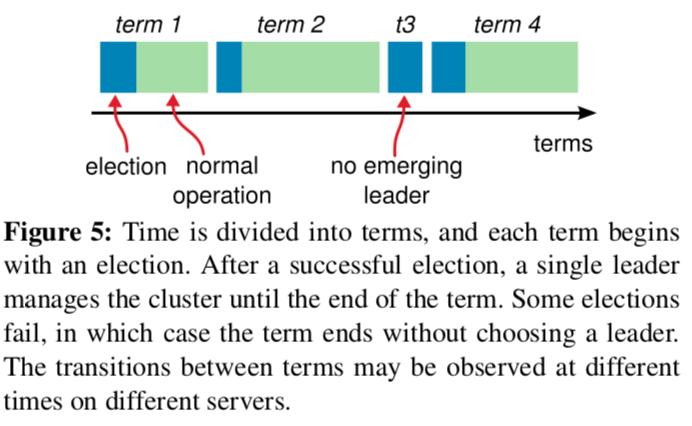
\includegraphics[width=1\linewidth]{./fig5.png}
%\caption{default}
%\label{default}
\end{center}
\end{figure}

在不同的时间,不同的servers可能观察到迁移发生在不同的任期。一些特殊的情况下,一个server可能观察不到一次选举或者某个任期。Raft中的任期表现的像逻辑锁,这些逻辑锁可以使得servers观察到某个leader是否已经过期。每个server都用一个变量存储了当前任期,并且这个变量随着时间是单调递增的。当servers进行通讯的时候,也会交换当前的任期。如果一个server存储的任期小于其他机器存储的任期,那么它将更新自己的任期到其它机器存储的最大任期。如果是一个候选者或者leader发现自己的任期已经过期,它们会转变到参与者的状态。如果一个server接受到一个请求,这个请求中的任期是过时的,它将直接拒绝该请求。

不同服务间的Raft模块是通过RPC进行通信的,Raft的简单版只需要两种类型的RPC。RequestVote RPCs是候选在这选举过程中使用的,AppendEntries RPCs是leader进行日志复制和心跳时使用的。在第七节我们增加了传送快照的RPC。所有的RPC请求在规定的时间没有接受到响应可以进行重试,这些请求在发送的时候可以并行进行从而获得更好的性能。

\subsection{选主}
Raft使用心跳机制来触发选主的过程。当servers启动的时候,都是作为参与者。如果一个参与者收到来自leader或者候选者的合法请求,它将保持在参与者的状态。leader会发送心跳到其它的server来授权延长自己的任期。如果一个参与者的选举定时器超时的时候还没有收到任何请求,它可以假设整个集群没有可用的leader或者候选者,然后发起新的选举。


一次选举开始时,参与者增加自己本地存储的当前任期然后转变为候选者状态。这个候选者先选举自己,并行的给集群中的其它机器发送RequestVote RPCs。候选者将会一直保持候选状态直到下面三件事情中的任意一件发生:(a):候选者本次选举胜出,(b):另外一台机器确认自己是leader,(c):僵持一段时候没有人胜出。上面的三种情况将在下面的段落进行讨论。


一个候选者如果接受到集群中大多数机器在同一个任期的选票,么它将胜出成为leader。每台机器在一个任期只能投票给一个候选者,按照先到先服务的原则(5.4节会对这个规则增加一些额外限制)。大多数投票胜出规则可以保证在一个特定的任期至多选出一个leader(图3所描述的选举安全原则)。一旦一个候选者胜出将成为集群的leader,它将会并行的给集群的其它机器发送心跳来宣示自己胜出,并阻止进行新的选举。


在等待选票的过程中,一个候选者可能接受到来自其它server的请求,该请求声明自己已经成为leader。如果请求中的leader的任期大于候选者本地存储的任期,那么当前候选者认为这个leader是合法的并转变为参与者状态。如果请求中leader的任期小于当前候选者本地存储的任期,那么候选将拒绝这个请求并保持在候选者状态。


第三种可能是是整个集群的所有候选者都没有胜出。如果集群中所有的参与者同一时刻转变为候选者,由于每个机器只能投票给一个候选者,这种情况新会很容易发生选举分裂即没有一个候选者获得半数以上选票。当这种情况发生,所有的候选者的选举定时器将会超时,它们增加自己本地存储的任期并启动新一轮的选举。从上面可以看出如果没有额外的规则约束,选举分裂的情况将极易发生。

Raft通过随机选举定时器来阻止选举分裂的发生,即使选举分裂发生也可以很快的被解决。选举超时将在[150,300]ms之间随机生成,这样就大概率保证集群中会有一个机器会先超时,而避免所有机器同时超时从而降低选举分裂情况发生的概率。如果首先超时的机器将会首先转变为候选者,它将会大概率的选举胜出成为leader,然后发送心跳续阻止其它机器定时器超时。9.3节讲述这种机器是有效的。
\begin{figure}[htbp]
\begin{center}
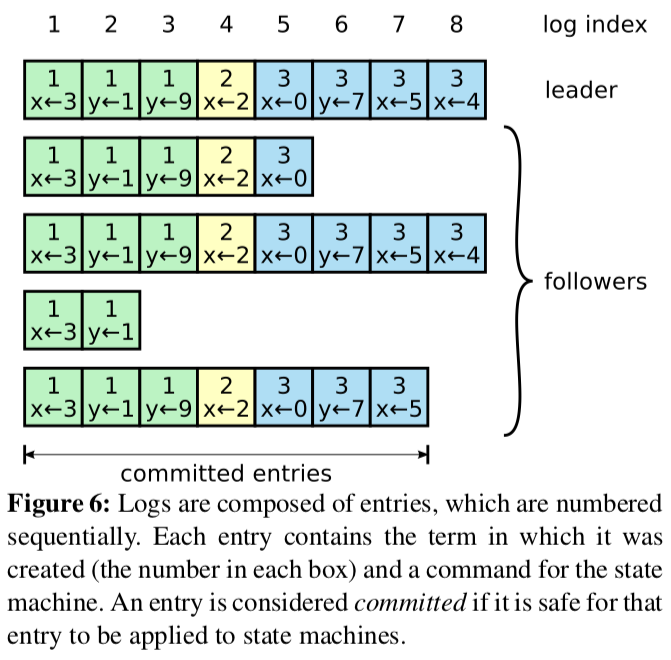
\includegraphics[width=1\linewidth]{./fig6.png}
%\caption{default}
%\label{default}
\end{center}
\end{figure}


选主的设计就是我们为了易懂而权衡的一种结果。最初我们准备使用一种给每个候选者加权的排名系统。这样当候选发现发现有别的候选者排名高于自己,它将转变为参与者从而保证排名高的候选者可以在下一轮以大概率胜出。但是排名的方法设计的更精巧而不是易懂,如果一个高排名的机器宕机,那么低排名的机器要等待超时后才能再次成为候选者,但是这样会延长选主过程。我们为了解决上面的问题对排名方法进行了很多次的调整,每次调整都会有新的问题产生。最终我们选择了随机重试方法,这种方法更为直观和易于理解。

\subsection{日志复制}
一旦一个候选者成为leader,它将开始处理客户端的请求。客户端的每个请求包含了一条需要执行到状态机的命令。leader将命令追加到自己的日志记录,同时并发AppendEntries RPCs请求来进行日志复制。当日志安全的复制之后,leader将日志应用到自己的状态机并将结果返回给客户端。如果集群中有参与者宕机、处理速度慢、网络丢包等情况发生,leader将重试AppendEntries RPCs请求直到日志被安全的复制。

日志的格式如图6所示。每条日志记录包含了leader的任期和状态机命令。任期是为了检测日志之间的不一致,从而保证图3所示的某些性质。同时每条日志记录也会有一个索引记录其在日志中的位置。

leader来决定将一条日志应用到状态机的安全时机。这样的一条日志被称为\textbf{\textit{committed}}。Raft来保证日志的持久化并且所有已提交的日志将会都会被应用到状态机。一旦leader将一条日志成功的复制到集群的大多数机器,那么这条日志就是已提交状态(如图6 的entry7)。如果当前日志记录已提交,那么由前任leader或者当前leader创建的前继日志记录都会被提交。5.4会讨论当leader变更后的应用日志的一些问题,同时也会定义什么是安全的提交。leader维护了即将被提交的日志记录的索引,并把这个索引放在未来的AppendEntries RPCs请求中。当参与者从请求获知已提交的索引,它会将本地该索引的日志应用到状态机。

我们设计Raft来保证不同机器之间日志的高度一致,不仅仅是为了可以简化和预测系统的行为,更重要的是保证系统的安全。Raft保证了下面的几个性质,这些性质共同组成了图3中的\textbf{\textit{Log Matching Property}}:
\begin{itemize}
\item 如果两个日志的两条日志记录有相同的索引和任期,那么这两条日志记录中的命令必然也是相同的。
\item 如果两个日志的两条日志记录有相同的索引和任期,那么这两个日志中的前继日志记录也是相同的。
\end{itemize}

在一个给定的任期,leader创建的日志索引是递增不重复的,一旦日志某条日志创建后是不会改变它在日志中位置。上面的事实保证了第一个性质的成立。每次当leader发送AppendEntries RPCs请求的时候,请求中会包含当前正在复制的日志记录的直接前继的任期和索引,如果参与者在自己的日志中没有发现有相同任期和索引的日志记录,它将直接拒绝请求。上面描述的一致性检测保证第二个性质的成立。一致性检测的步骤如下:初始化时候是满足Log Matching Property的;当有追加日志的时候进行一次一致性检测来保护Log Matching Property。这样当leader接受到返回成功的AppendEntries RPCs请求时,说明了参与者与自己的日志是相同的。
\begin{figure}[htbp]
\begin{center}
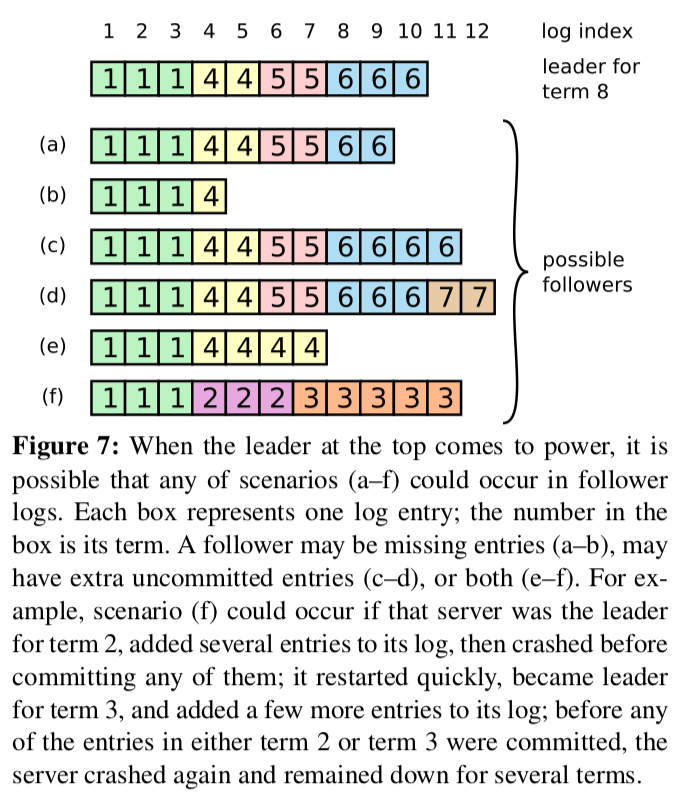
\includegraphics[width=1\linewidth]{./fig7.png}
%\caption{default}
%\label{default}
\end{center}
\end{figure}

正常情况下,leader和参与者的日志都是相同的,日志一致性检测也不失败。当leader崩溃的时候就会导致日志的不一致,例如旧的leader没有将自己的日志记录安全的复制到其它机器。这些不一致可能聚合多个leader和参与者的崩溃。图7描述参与者的日志和新leader日志不一致的情况。一个参与者可能缺失了leader有的日志记录,它也可能多出了leader没有的日志,或者上面的两种情况同时发生。缺失或多余的日志可能存在在多个任期。

Raft是通过强制参与者只能复制leader的日志来解决不一致。这就意味者参与者的日志和leader的日志发生冲突的时候,参与者的日志将会重写或者删除。5.4将会讨论在额外附加的约束下上面的过程是安全的。

如果一致性检测失败后,为了保证参与者和自己的日志一致,leader需要先确认参与者和自己一致的最后一条日志记录。然后通知参与者删除这条日志记录后面的日志,并将这条日志记录之后的日志复制给参与者。leader为每个参与者维护了\textit{nextIndex},这个索引记录了leader将复制给该参与者的日志索引。当一个leader选举生效后,它将初始化\textit{nextIndex}为它自己日志记录中最后一条日志记录的索引(图7索引11所示)。如果leader的日志和参与者的日志不一致那么下一轮的AppendEntries RPCs进行AppendEntries一致性检测的时候就会发现。如果检测发生不一致,leader将会减少\textit{nextIndex}并重试。经过多次重试leader就会确定参与者和自己一致的日志索引,然后通知参与者删除后面不一致的日志,然后复制自己的日志给参与者。经过上面的过程leader和参与者的一致就可以恢复一致。

上面过程中每次\textit{nextIndex}减少1进行重试效率是存在问题的,但是也是可以优化的。一旦参与者进行日志一致性检测发现不一致之后,在响应leader请求中包含自己在这个任期存储的第一条日志。这样leader接受到响应后,就可以直接跳过所有冲突的日志(其中可能包含了一致的日志)。这样就可以减少寻找一致点的过程。但是在实际中我们怀疑这种优化的必要性,因为失败发生的概率本来就很低,也不会同时存在大量不一致的日志记录。

使用上面的机制,一个leader生效的时候就不需要进行额外的操作来恢复日志的一致性。它只需按照正常的流程,日志的不一致经过多次AppendEntries RPCs一致性检测后会自动收敛。leader也不需要重写和删除本地日志(图3的日志只追加特性)。

上面所描述的日志复制机器满足了第2节所期望的一致性特性:Raft可以在集群只有半数以上存活的情况下接受、复制和应用新的日志记录;正常情况下只需要一轮RPCs可以将日志记录复制到集群的大多数;单个速度慢的参与者不会影响整个集群的性能。

\subsection{安全性}
之前的章节描述了Raft的选主和日志复制。但是目前所描述的机制还不能安全的保证日志是按照相同顺序被应用到状态机。例如:在leader提交了若干条日志后,某个参与者宕机并被选为新的leader。新的会leader重写其它机器的日志,结果导致不同的状态机有不同的命令序。

我们通过添加额外约束控制某些机器能被选举为leader来完善Raft算法。这个约束保证当选的leader包含了前任所有提交的日志(图3的Leader Completeness Property)。通过约束我们可以精准的控制日志的提交。这节剩下的部分我们会给出Leader Completeness Property一个简略的证明,并解释它如何保证复制状态机的正确性。

\subsubsection{选举约束}
在基于leader的一致性算法,leader最终会存储所有已提交的日志记录。在某些一致性算法中,一个日志即使没有存储所有已提交的日志也可以称为leader。这些算法会通过额外的机制来确定缺失的日志然后传给新的leader,上面的过程可能发生在选举过程或者选举胜出后。不幸的是,这样会增加额外的复杂度。Raft使用的方法是每个当选的leader必须之前所提交的所有日志,这种方法不需要复制日志到新当选的leader。这种方法带来的好处是集群中数据的流向只能是从leader到参与者,leader永远仅需要追加即可。

\begin{figure}[htbp]
\begin{center}
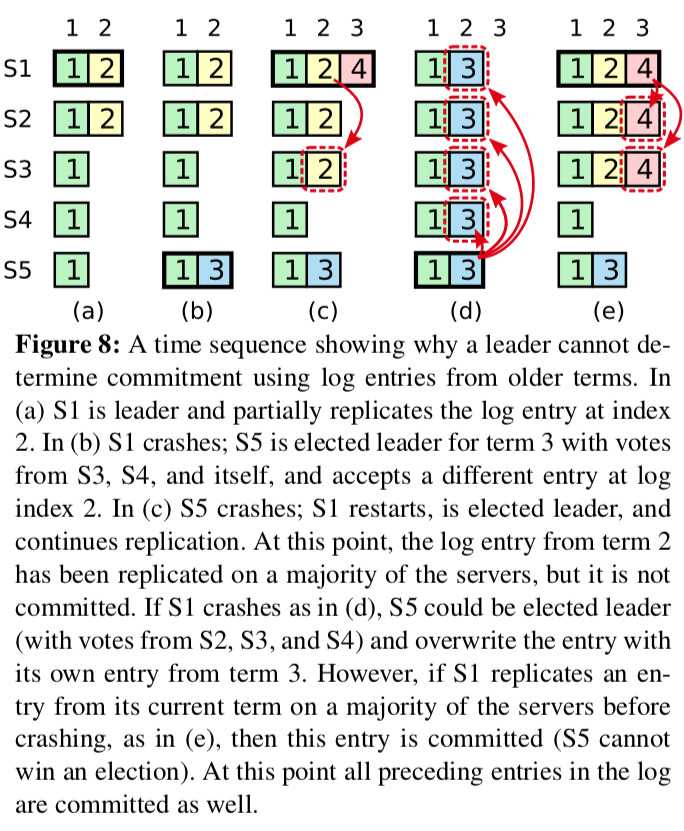
\includegraphics[width=1\linewidth]{./fig8.png}
%\caption{default}
%\label{default}
\end{center}
\end{figure}

Raft使用选举过程来保证一个候选者必须包含有所有已提交的日志才能胜出。候选者为了胜出必须联系集群中的大多数机器,这就意味着每条日志至少出现在机群中的某一台机器上。如果候选者的日志如果比集群其它任意一台机器的日志更新(下面精确定义“更新”),那么它将包含所有已提交的日志。RequestVote RPCs来实现这个约束:请求中包含了leader的日志信息,如果投票者的日志比候选者的日志更新,那么它就拒绝投票。

两个日志文件谁的日志更新是通过比较日志中最后一条日志记录的任期和索引。如果两个日志文件的最后一条日志的任期不相同,谁的任期更大谁的的日志将更新。如果两条日志记录的任期相同,那么谁的索引越大,谁的日志将更新。

\subsubsection{提交上一个任期的日志}

如第5.3描述,如果当前任期的一条日志已经被复制到集群中的大多数,那么leader可以确定这条已经已经处于提交状态。如果上任leader在提交日志之前宕机,下一任leader将尝试完成日志的复制。然而,尽管上一任期的某条日志已经被复制到了大多数机器,但是新任leader还是不能准确断定这条日志是否是已提交。图8展示了这样一种情况。
\begin{figure}[htbp]
\begin{center}
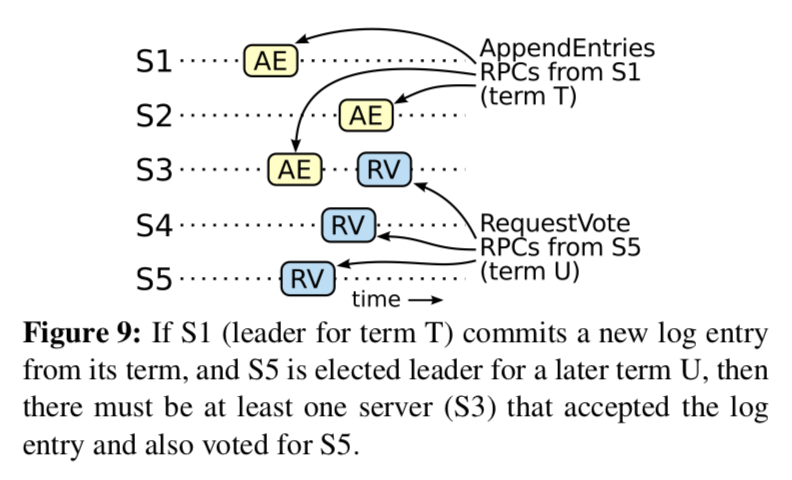
\includegraphics[width=1\linewidth]{./fig9.png}
%\caption{default}
%\label{default}
\end{center}
\end{figure}

为了消除如图8所示的问题。Raft不能根据上一任期的日志是否被复制到大多数机器来决定是否提交日志。一旦当前任期看到一条日志被提交,由于Log Matching Property保证,那么这条日志之前的日志已自动被提交。有一些情况下,一个leader可以安全的断定一条老的日志是否已提交(例如一条日志已经被存储在所有的机器上),但是Raft采取了保守的方法来使得问题简化。

Raft在提交过程引入的额外复杂度是因为前一个任期已经复制的日志保持了它原来的任期编号。在一些其它的一致性算法中,如果一个新的leader复制复制前面任期的日志,那么之前的任期编号必须转换为当前的任期编号。Raft的方法使日志记录变的简单,同一个任期编号可以跨越时间和日志文件。除此之外,在复制前任的日志记录下,新的leader需要更少次数的复制相比其它一致性算法(在日志提交前,其它一致性算法需要复制冗余的日志记录来变换任期编号)。

\subsubsection{安全讨论}

给出了完整Raft算法,我们可以更精确的讨论Leader Completeness Property(这里的讨论基于安全的证明,参看9.2节)。我们假设Leader Completeness Property不成立,使用反证法证明Leader Completeness Property成立。假设任期T的leader在它的任期提交了一条日志,但是这条日志并没有被复制到未来某个任期的leader。考虑大于T的最小任期U没有存储这条日志。

\begin{description}
\item[1.]当任期U的leader在它选举的时候这条已提交,日志已不存在于它的日志中(leaders没有删除或者覆写)。
\item[2.]任期T的leader已经将日志复制到大多数机器,同时任期U的leader也接受到集群大多数机器的选票。那么至少存在一台机器即接受到任期T的leader复制的日志同时也投票给任期U的leader,如图9
所示。这个投票者是反证法的关键。
\item[3.]这个投票者一定是先接受任期T的leader复制日志,然后投票给任期U的leader。否则它将拒绝来自任期T的leader的AppendEntries请求(否则它的任期将大于T,与假设矛盾)。
\item[4.]这个投票者投票给任期U的leader的时候,已经存储了这条日志,因为这中间任期的leader包含这条日志(通过假设),leaders没有删除过这条日志,参与者只删除自己和leader冲突的日志。
\item[5.]投票者将自己的票投给任期U的leader,所以任期U的leader的日志一定和自己的一样新。这将推出两个矛盾中的一个。
\item[6.]首先,如果投票者和任期U的leader的最后一条日志记录相同,那么任期U的leader的日志至少和投票者的日志一样长,所以它的日志包含了投票者的所有日志。这也是一个矛盾,因为投票者包含了已提交的日志,而我们假设任期U的leader没有这条日志。
\item[7.]否则,任期U的leader的最后一条日志必须大于投票者。进一步,同时也大于任期T,因为投票者最后一条日志的任期至少是T(它存储了来自任期T的日志)。创建任期U的leader最后一条日志的任期leader,一定包含这条已提交的日志(通过假设)。那么,根据性质Log Matching Property,任期U的leader也一定包含这条已提交的日志,这是一个矛盾。
\item[8.]这里完成反证法。所以任期大于T的任期一定包含在任期T提交的所有日志。
\item[9.]Log Matching Property保证未来的leader也包含已经提交的日志,图8(d)index 2所示。
\end{description}

证明Leader Completeness Property,我们可以证明图3中的State Machine Safety Property。这条性质是讲如果一台机器已经应用一条给定索引的日志记录到状态机,其他机器将不会应用一条具有相同索引但是内容不同的日志到状态机。只有在和leader的日志相同的情况下并且这条日志已经提交,参与者参会将这条日志记录应用到自己的状态机。考虑任何一台机器应用了一条给定的索引在最小的任期;Log Matching Property将会保证大于最小任期的leader都包含这条指定索引的日志记录。所以servers在最新的任期应用这条日志将有相同的值。所以State Machine Safety Property成立。

最终,Raft需要servers按照日志索引顺序将应用日志到状态机。结合State Machine Safety Property性质,那么所有的servers将按照相同的顺序执行相同的日志到状态机。


\subsubsection{参与者和候选者宕机}
目前为止我们都是聚焦在leader不可用,参与者和候选者采用比leader简单的方法处理不可用。如果参与者或者候选者不可用,那么发送给他们的RequestVote和AppendEntries RPCs将会失败,然后Raft采用重试的策略;如果宕机重启,那么重试的请求将会成功。如果一个机器还没有来的及回应就宕机,再它重启之后将会接受和宕机前相同的请求。Raft请求是可重入的,重试是没有危害的。举个例子,如果候选者接受的AppendEntries请求中日志已经被存储们,直接忽略这些请求。

\subsubsection{时基和可用性}
Raft安全性一个要求就是不能依赖时间:系统不能由于某些事件发生比期望快或者慢就导致不正确的结果。然而,系统可用性不可避免的会依赖时间。例如:如果一条消息交换的时间长于机器宕机间隔,候选者不能存活足够长的时间去赢得选举;如果没有一个稳定的leader,Raft将不能工作。

选主是Raft的一部分,其中时间是至关重要的。Raft可以进行选举和保持一个稳定的leader,需要系统满足下面的时间要求:
\begin{center}
\textit{broadcastTime <<  electionTimeout  << MTBF} 
\end{center}
这个不等式中的broadcastTime是一个server并行发送RPCs到每个机器并接受到它们回应的平均时间;
 electionTimeout是5.2描述的选举超时时间;MTBF单台机器的平均故障间隔时间。broadcastTime的数量级必须远远小于electionTimeout,这样leader才可以可靠的发送心跳来阻止参与者启动新的选举;选定超时时间通过使用随机化的方法,这个不等式可以保证选举分裂发生的概率很小;election timeout也应该在数量级上远远小于MTBF,这样系统才能稳定的运行。当leader 宕机,系统最长不可用时间不会超过选举超时时间,我们可以预想到不可用时间占整个运行时间极小的一部分。
 
broadcastTime和MTBF是下伏系统的固有特性,我们能选择的只有选举超时时间。Raft的RPCs请求往往需求接受者将信息持久化到稳定存储介质,所以broadcastTime会在0.5ms到20ms之间波动。
\begin{figure}[htbp]
\begin{center}
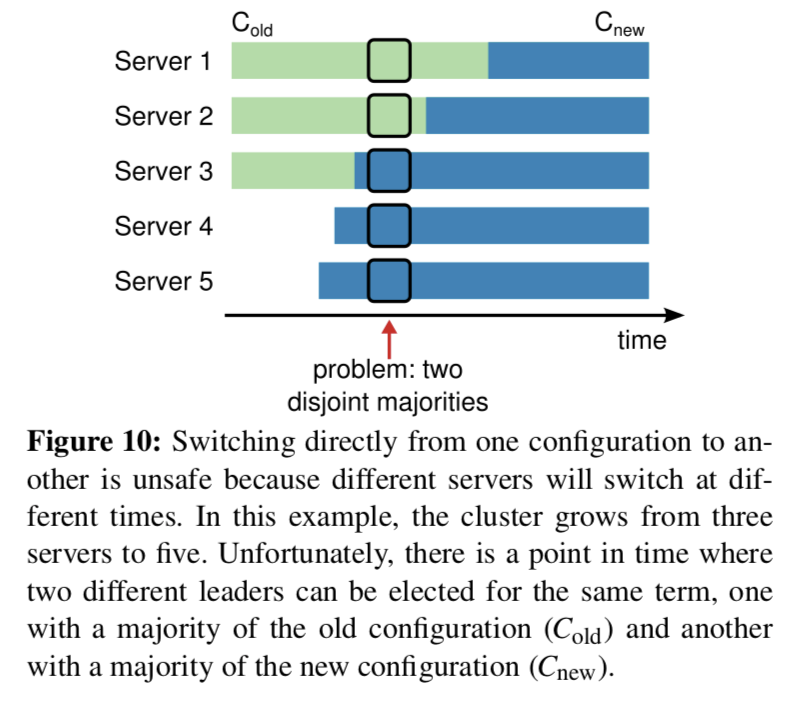
\includegraphics[width=1\linewidth]{./fig10.png}
%\caption{default}
%\label{default}
\end{center}
\end{figure}
根据上面的分析,选举超时时间应该在[10ms,500ms]。典型的MTBF往往是数月或者更久,可以轻松满足系统的时间需求。


\section{集群成员变更}
目前为止我们都是假定集群的配置(参与一致性算法的机器集合)是固定的。在实际系统中,我们有时候可能需要变更配置,例如需要替换宕机的机器或者增加日志的副本数。最笨的方法,我们可以停掉整个集群更换配置并重启集群,但是这将导致整个集群不可用。除此之外,手工操作也会带来其它的风险。最终Raft决定支持配置的热变更。

如果要保证配置变更过程是安全的就要保证变更过程中同一个任期不可能有两个leader选举胜出。不幸的是,所有直接从旧配置切换到新配置方法都是不安全的。同一时刻切换所有的机器是不可能的,所以变更过程中,集群可以分裂成两个部分(如图10所示)。

为了保证安全,配置变更采用两阶段的方法。这里有很多方法可以实现两阶段,例如:有的系统在第一个阶段来停止旧配置,这样就不能响应客户端的请求;然后第二阶段切换到新配置。Raft集群第一阶段会过渡到迁移配置(我们称之为联合一致性配置joint consensus);一旦联合一致性被提交,系统将切换到新配置。joint consensus配置组合了老配置和新配置。
\begin{itemize}
\item 日志记录将被复制新老配置到所有机器。
\item 新老配置的机器都可以作为leader。
\item 表决(选举或是日志提交)同时需要老配置中的多数派和新配置中的多数派同意。
\end{itemize}

\begin{figure}[htbp]
\begin{center}
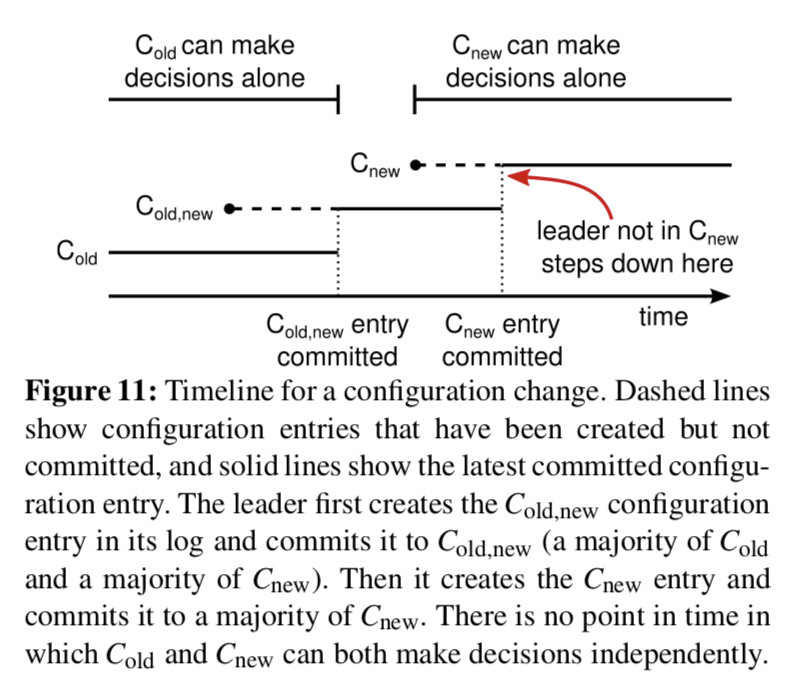
\includegraphics[width=1\linewidth]{./fig11.png}
%\caption{default}
%\label{default}
\end{center}
\end{figure}
联合一致性允许独立的机器变更在不同的配置而不需要保证安全性。进一步,联合一致性可以允许集群在配置变更过程中处理客户端的请求。

集群的配置存储和交换是通过特殊的日志进行的。图11展示配置的交换过程。当leader接受到请求要将配置从老配置切换到新配置,它将存储联合一致性配置,并通过日志复制将联合一致性日志复制到其它机器。一旦一个参与者接受将这条日志记录并写入自己的日志中,它将使用这个配置来进行后面的决策(一个机器永远使用最新的配置进行决策,不管这条日志记录是否提交)。这就意味这leader将使用联合一致性配置的来决策日志是否提交。如果leader 宕机,一个新的leader将会被选举,可能是旧配置也可能是新配置,依赖于候选者是否接受到联合一致性配置。在任何情况下,新配置不能单边作出决定在配置的变更期间。

一旦联合一致性配置已经被提交,不管老配置还是新配置都不可能在不得到对方支持的情况下作出决策,Leader Completeness Property保证那些使用联合一致性配置的机器可以被选作leader。那么ledaer就可以安全的创建一条日志对于新配置,并将配置复制到其它机器。此外,这个配置一旦被机器接受到就会立即生效。当新的配置在新配置的规则下被提交,那么老配置将变得无关紧要,不在新配置中的机器就可以停机下线了。如图11所示,这里存在新配置和老配置同时作出单边决定的时刻。这样就保障了安全性。

配置变更中有三个问题需要说明。第一个问题就是新的机器初始化的时候可能不存储任何日志。如果它们以这样的状态加入集群,需要花费很长的时间后它们的日志才能追赶上集群中其他机器。在这个期间集群是不能提交新的日志。为了避免不可用间隙,Raft在配置变更前引入了一个新的阶段,在这个阶段新加入的机器没有表决权(leader将日志复制给它们,但是它们不是投票集合的成员)。一旦新机器的日志追赶上集群的其它机器,配置的变更就可以如前面描述的过程进行。

第二个问题是leader可能不是新配置的机器。这种情况下,leader在提交新配置下的日志记录后就降级到参与者状态。这就意味这存在一时间leader管理着一个不包含自己的集群;也就是说它仅仅复制而它自己不是表决集合的成员。leader的变更发生在新配置被提交,因为是从这个时间点新配置可以单独的运行。在这个点之前,可能都是老配置的机器被选举为leader。

第三个问题就是删除机器(不在新配置中的机器),这些机器可能中断集群。这些机器接受不到心跳,所以它们就会超时重启新的选举。它们会发送携带新任期编号的RequestVote RPCs,这将会造成当前leader回退到参与者状态。一个新的leader虽然会被选举,但是需要移除的机器将会再次超时,这个过程将不断重复,导致集群的频繁不可用。

为了阻止第三个问题的发生,servers在确定leader存在的情况下将不理会RequestVote RPCs。特殊地,如果一个机器在最小超时时间下接受到来自当前任期leader的RequestVote RPC,它将不更新自己的任期,也不参与这次投票。这不会影响正常的选举,这里每个机器直到等待一个最小超时时间在新一轮的选举之前。然而,这样会阻止待移除的机器扰乱整个集群:如果一个leader可以接受到当前集群的心跳,它将不会被更大任期的所废除。

\section{日志压缩}
随着集群的运行,机器的日志将会不断增长。在实际系统中,日志不可能无限增长。日志不断增长将会占据更多的空间,花费更多的时间进行回放。为了保证集群的可用性需要额外的机制来删除日志中过期的日志。
\begin{figure}[htbp]
\begin{center}
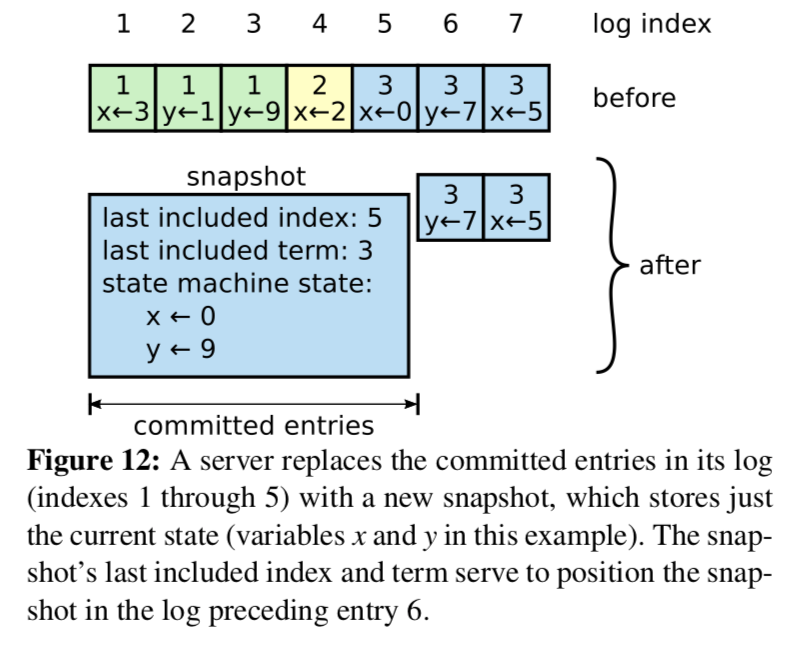
\includegraphics[width=1\linewidth]{./fig12.png}
%\caption{default}
%\label{default}
\end{center}
\end{figure}

快照是最简单的压缩方法。快照方法下,当前整个系统状态将会写到存储在稳定存储介质的一个快照。这样这个点之前的日志就可以删除。快照被使用在Chubby和ZooKeeper中,接下来的章节我们将会描述Raft中的快照。

使用递增的方法进行压缩,例如日志清理和LSM tree都是可以的。递增法压缩往往都是发生在少部分数据上,这将会导致系统需要进行频繁的压缩。它们首先选择一个有很多删除和重复数据的区块,然后将压缩后的内容写入到一个新的区块,并释放旧的区块从而实现日志的压缩。相比快照这需要额外的机制和复杂度来实现,而快照机制每次都是对整个数据集进行操作。如果使用日志清理那么就需要对Raft进行修改,状态机提供给LSM tree的接口快照同样可以使用。

图12展示了Raft中快照的基本思想。每个机器独立的进行快照,快照只需要覆盖已经提交的日志。更多的工作是状态机将自己的当前的状态写入到快照中。Raft包含了少量的metadata在快照中:last included index日志中最后一条被快照取代的日志的索引(也是状态机应用的上一条日志的索引)。 last included term是这条日志对应的任期。这些被持久化用来支持AppendEntries的日志一致性检测,如前面讲述的日志一致性检测需要前一条日志的任期和索引。为了支持集群成员变更(第六节),快照也包含了最后一条被快照取代的日志所使用的配置。一旦机器完成快照,它将可以删除last included index之前的所有日志,也包括之前的快照。


正常情况下机器都是单独的进行快照,但是某些情况下leader也会发送快照到那些落后的机器上。上面的情况发生在leader已经删除了下条需要发送给参与者的日志记录。幸运的是,这种情况在正常操作下不会发生:一个参与者保持和leader有一样的日志。然而,一个异常慢的参与者或者一个新的机器加入到集群,这些情况下leader就需要通过网络发送快照来使其它的机器追赶上自己。



\begin{table}[htp]
\begin{center}
\begin{tabular}{|p{2.5cm}p{5.5cm}|}
\hline
\multicolumn{2}{|c|}{\textbf{InstallSnapshot RPC}}  \\
\hline
\multicolumn{2}{|l|}{\textbf{被用来复制快照到参与者:}} \\
&\\
\multicolumn{2}{|l|}{\textbf{Arguments:}} \\
\textbf{term} & leader的任期\\
\textbf{leaderId} & 参与者重定向到leader\\
\textbf{lastIncludedIndex} & 快照替换的最后一条日志记录的索引 \\ 
\textbf{lastIncludedItem} & 快照替换的最后一条日志记录的索引的任期 \\
\textbf{offset} & 快照中块的字节偏移量 \\
\textbf{data[]} & 数据块,从偏移量开始存储 \\
\textbf{done} & 是否是最后一个块文件 \\
&\\
\multicolumn{2}{|l|}{\textbf{Results:}} \\
\textbf{term} & 当前任期,leader用来更新自己\\

&\\
\multicolumn{2}{|l|}{\textbf{接受者的实现:}} \\
\multicolumn{2}{|l|}{1. 如果leader的任期小于自己的任期返回false。} \\
&\\
\multicolumn{2}{|l|}{2. 创建新的快照文件,如果是第一个块文件(偏移量为0)。} \\
&\\
\multicolumn{2}{|l|}{3. 在快照文件的指定偏移量写入数据。}\\
&\\
\multicolumn{2}{|l|}{4. 如果done为假,等待更多的块数据。}\\
&\\
\multicolumn{2}{|l|}{5. 保存快照文件,删除快照之前的日志。}\\
&\\
\multicolumn{2}{|l|}{6. 如果存在快照点之后日志日志,保留这些日志并重放。}\\
&\\
\multicolumn{2}{|l|}{7. 删除整个日志文件。}\\
&\\
\multicolumn{2}{|l|}{8. 使用快照的状态重置状态机,并加载快照中的配置。}\\
&\\
\hline
\multicolumn{2}{l}{}\\
\multicolumn{2}{l}{Figure 13: A summary of the InstallSnapshot RPC. Snap-}\\
\multicolumn{2}{l}{\qquad \qquad shots are split into chunks for transmission; this gives}\\
\multicolumn{2}{l}{\qquad \qquad the follower a sign of life with each chunk, so it can} \\
\multicolumn{2}{l}{\qquad \qquad  reset its election timer.}\\
\end{tabular}
\end{center}
\label{default}
\end{table}%

leader将会使用一种叫做InstallSnapshot新的RPC来拷贝快照到那些远远落后的机器。如图13所示,当一个参与者接受一个包含快照的RPC,它必须决定对已经存在的日志进行处理。通常快照会包含接受这日志中没有的新信息。这种情况下,参与者删除整个日志并被快照取代,如果参与者重复接受到一个快照,那么快照之前的日志记录可以删除,但是快照之后的日志记录是合法的并需要被保留。

这种快照法有悖Raft的强领导原则,因为参与者可以在没有leader情况下进行快照。然而,我们认为这样的背离是合理的,存在leader是为了避免冲突并达成一致,快照的时候一致性已经达成,所以没有决定是冲突的。集群中的数据流依旧是从leader流向参与者,只是参与者可以重组自己的数据。

我们认为基于强领导的方法只有leader可以创建快照,然后将快照复制给其它的参与者。然而这里存在两个缺点。第一个,通过网络发送快照将会浪费网络带宽,拖慢快照的处理速度。每个参与者已经具备了产生快照的所有信息,一个参与者通过自己的状态机产生快照的成本是远远低于来自leader的快照。第二,这样将会使leader的实现变的复杂。例如:leader可以在并发复制新的日志的时候发送快照,这样将不会阻塞来自客户端的新的请求。

这里有两个方面制约快照的速度。第一,机器需要决定什么时候进行快照。如果一个机器快照的频率过高将会浪费磁盘的带宽和能力;如果快照频率过慢将会加剧容量不足的风险,也会增加重放日志的耗时。一个简单的策略是当日志的总量达到某个阈值的时候进行快照。如果这个阈值设置的比较大,这样快照耗费的磁盘就会比较小。

第二制约性能的问题是快照快照要花费很长的时间,我们不希望拖慢正常的操作,我们可以接受拖慢非正常操作。解决方法就是使用写时复制技术,在进行快照的同时也可以接受新的更新。例如:使用结构化数据设计的状态机天然的支持写时复制。此外,我们可以使用操作系统的写时复制技术来创建基于内存的整个状态机的快照(我们的实现采用了这种方法)。

\section{客户端交互}

这一章节我们将描述Raft是如何和客户端交互的,包含客户端如何发现集群的leader以及Raft支持线性语义。这些技术在所有基于一致性的系统中都有应用,Raft的方案和其它系统的相似。

Raft的客户端将自己的请求发送到leader。当一个客户端首次启动,它会随机的选择集群的一台机器。如果客户端的首次选择不是leader,这台机器将拒绝客户端的请求,并会告知自己最近监听到的leader。如果leader宕机,客户端的请求将会超时,客户端可以随机的选择机器进行重试。

Raft的目标是实现线性语义(每个操作都是立刻被执行的),然而,目前为止我们描述的Raft可以重复多次的执行一条命令;例如,如果leader提交了日志但是还没有来得及响应客户端就宕机,那么客户端将会换一个leader重试之前的命令。解决方法就是客户端给每个命令一个唯一的编号,那么,状态机记录每个客户端处理的最新的编号。一旦接受到一条命令它的序列号已经被执行过,直接响应这个请求但是不重新执行这个请求。

只读操作可以阻止日志的写入。然而没有额外的机制会增加返回脏数据的风险,因为leader响应的请求可能被一个新的不知情的leader废除。线性读不能返回脏数据,Raft需要两个额外的措施来保证而不是通过使用日志。第一,一个leader必须知道被提交的日志记录的最新信息。 Leader Completeness Property保证leader拥有所有已提交的日志,但是任期刚开始的时候,它可能不知道那些是已提交的。为了弄清楚,它需要在自己的任期提交一条日志。Raft通过让每个leader提在自己刚当选的时候提交一个空操作的日志记录到自己的日志。第二,一个leader在处理一个只读日志之前必须检测自己是否被废除(如果最近一个新的leader已经被选举,那么它的信息可能是过时的),Raft需要在响应只读请求之前需要leader和半数以上的机器交换心跳信息。或者,leader可以依靠心跳值来提供租约,但是这样会使安全依赖于时间(因为这里假定有界始终偏移)。

\section{实现和评估}
我们实现了Raft用来复制RAMCloud的配置信息和支持RAMCloud失败协调。我们大约使用了2000行C++代码。我们实现的代码已经开源,这里还有25独立的第三方机构的开源实现,不同的公司也部署了基于Raft的系统。
下面的章节通过三方面评估Raft协议:易理解性、正确性和性能。

\subsection{Understandability}
To measure Raft’s understandability relative to Paxos, we conducted an experimental study using upper-level un- dergraduate and graduate students in an Advanced Oper- ating Systems course at Stanford University and a Dis- tributed Computing course at U.C. Berkeley. We recorded a video lecture of Raft and another of Paxos, and created corresponding quizzes. The Raft lecture covered the con- tent of this paper except for log compaction; the Paxos lecture covered 
enough material to create an equivalent replicated state machine, 
including single-decree Paxos, multi-decree Paxos, reconfiguration, and a few optimiza- tions needed in practice (such as leader election). 
\begin{figure}[htbp]
\begin{center}
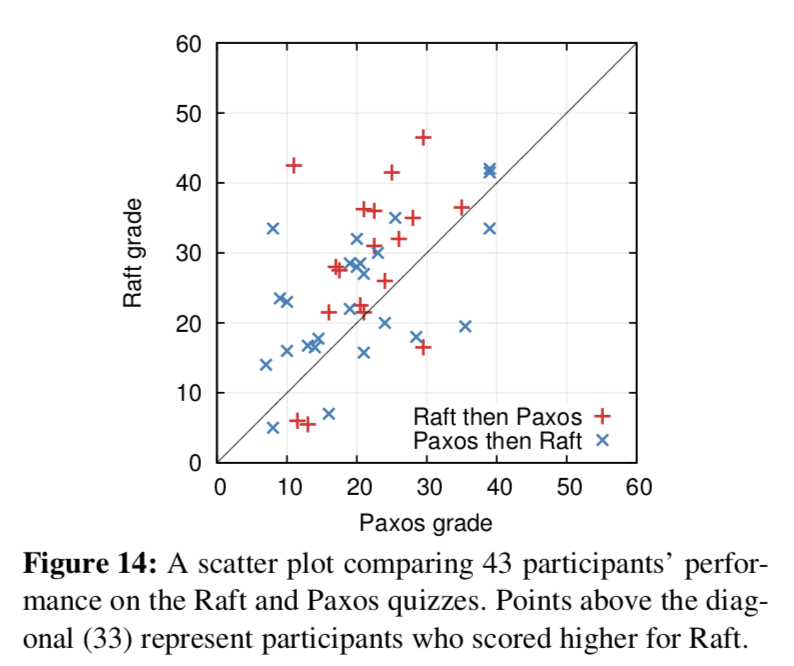
\includegraphics[width=1\linewidth]{./fig14.png}
%\caption{default}
%\label{default}
\end{center}
\end{figure}
The quizzes tested basic understanding of the algorithms and also required students to reason about corner cases. Each student watched one video, took the corresponding quiz, watched the second video, and took the second quiz. About half of the participants did the Paxos portion first and the other half did the Raft portion first in order to account for both individual differences in performance and experience gained from the first portion of the study. We compared participants’ scores on each quiz to deter- mine whether participants showed a better understanding of Raft.

We tried to make the comparison between Paxos and Raft as fair as possible. The experiment favored Paxos in two ways: 15 of the 43 participants reported having some prior experience with Paxos, and the Paxos video is 14\% longer than the Raft video. As summarized in Table 1, we have taken steps to mitigate potential sources of bias. All of our materials are available for review [28, 31].

On average, participants scored 4.9 points higher on the Raft quiz than on the Paxos quiz (out of a possible 60 points, the mean Raft score was 25.7 and the mean Paxos score was 20.8); Figure 14 shows their individual scores. A paired t-test states that, with 95\% confidence, the true distribution of Raft scores has a mean at least 2.5 points larger than the true distribution of Paxos scores.

\begin{figure}[htbp]
\begin{center}
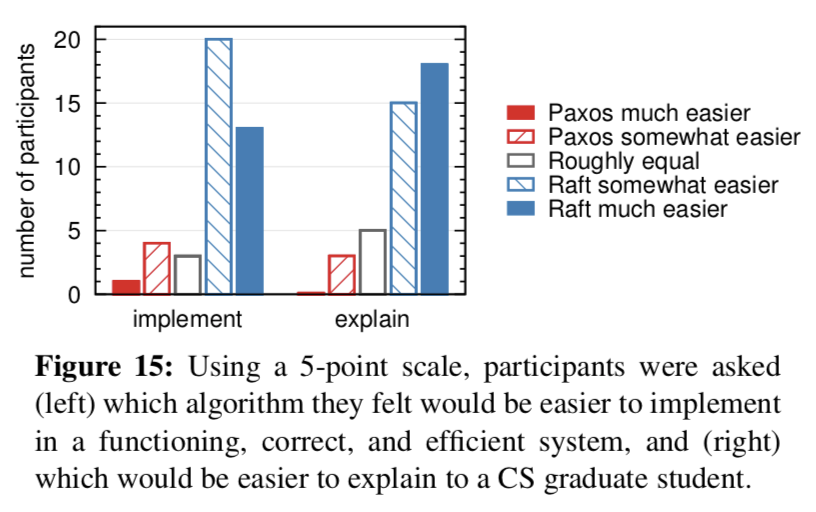
\includegraphics[width=1\linewidth]{./fig15.png}
%\caption{default}
%\label{default}
\end{center}
\end{figure}
We also created a linear regression model that predicts a new student’s quiz scores based on three factors: which quiz they took, their degree of prior Paxos experience,  which they learned the algorithms. The model predicts that the choice of quiz produces a 12.5-point dif- ference in favor of Raft. This is significantly higher than the observed difference of 4.9 points, because many of the actual students had prior Paxos experience, which helped Paxos considerably, whereas it helped Raft slightly less. Curiously, the model also predicts scores 6.3 points lower on Raft for people that have already taken the Paxos quiz; although we don’t know why, this does appear to be sta- tistically significant.

We also surveyed participants after their quizzes to see which algorithm they felt would be easier to implement or explain; these results are shown in Figure 15. An over- whelming majority of participants reported Raft would be easier to implement and explain (33 of 41 for each ques- tion). However, these self-reported feelings may be less reliable than participants’ quiz scores, and participants may have been biased by knowledge of our hypothesis that Raft is easier to understand.
A detailed discussion of the Raft user study is available at [31].

\subsection{Correctness}

We have developed a formal specification and a proof of safety for the consensus mechanism described in Sec- tion 5. The formal specification [31] makes the informa- tion summarized in Figure 2 completely precise using the TLA+ specification language [17]. 
\begin{figure}[htbp]
\begin{center}
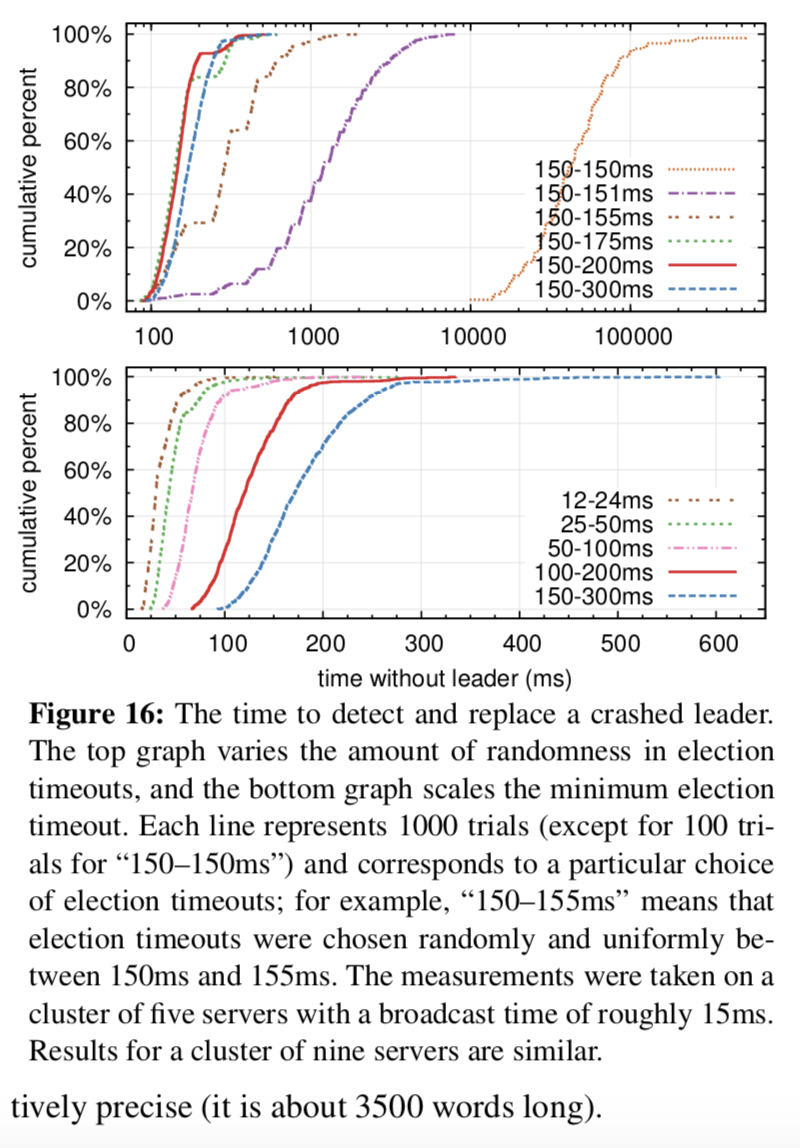
\includegraphics[width=1\linewidth]{./fig16.png}
%\caption{default}
%\label{default}
\end{center}
\end{figure}
It is about 400 lines long and serves as the subject of the proof. It is also use- ful on its own for anyone implementing Raft. 
We have mechanically proven the Log Completeness Property us- ing the TLA proof system [7]. However, this proof relies on invariants that have not been mechanically checked (for example, we have not proven the type safety of the specification). Furthermore, we have written an informal proof [31] of the State Machine Safety property which is complete (it relies on the specification alone) and rela-tively precise (it is about 3500 words long).

\subsection{Performance}
Raft’s performance is similar to other consensus algo- rithms such as Paxos. The most important case for per- formance is when an established leader is replicating new log entries. Raft achieves this using the minimal number of messages (a single round-trip from the leader to half the cluster). It is also possible to further improve Raft’s per- formance. For example, it easily supports batching and pipelining requests for higher throughput and lower la- tency. Various optimizations have been proposed in the literature for other algorithms; many of these could be ap- plied to Raft, but we leave this to future work.

We used our Raft implementation to measure the per- formance of Raft’s leader election algorithm and answer two questions. First, does the election process converge quickly? Second, what is the minimum downtime that can be achieved after leader crashes?

To measure leader election, we repeatedly crashed the leader of a cluster of five servers and timed how long it took to detect the crash and elect a new leader (see Fig- ure 16). To generate a worst-case scenario, the servers in each trial had different log lengths, so some candidates were not eligible to become leader. Furthermore, to en- courage split votes, our test script triggered a synchro- nized broadcast of heartbeat RPCs from the leader before terminating its process (this approximates the behavior of the leader replicating a new log entry prior to crash-ing). The leader was crashed uniformly randomly within its heartbeat interval, which was half of the minimum election timeout for all tests. Thus, the smallest possible downtime was about half of the minimum election time- out.


The top graph in Figure 16 shows that a small amount of randomization in the election timeout is enough to avoid split votes in elections. In the absence of random- ness, leader election consistently took longer than 10 sec- onds in our tests due to many split votes. Adding just 5ms of randomness helps significantly, resulting in a median downtime of 287ms. Using more randomness improves worst-case behavior: with 50ms of randomness the worst- case completion time (over 1000 trials) was 513ms.

The bottom graph in Figure 16 shows that downtime can be reduced by reducing the election timeout. With an election timeout of 12–24ms, it takes only 35ms on average to elect a leader (the longest trial took 152ms). However, lowering the timeouts beyond this point violates Raft’s timing requirement: leaders have difficulty broad- casting heartbeats before other servers start new elections. This can cause unnecessary leader changes and lower overall system availability. We recommend using a con- servative election timeout such as 150–300ms; such time- outs are unlikely to cause unnecessary leader changes and will still provide good availability.

\section{Related work}

There have been numerous publications related to con- sensus algorithms, many of which fall into one of the fol- lowing categories:
\begin{itemize}
\item Lamport’s original description of Paxos [15], and at- tempts to explain it more clearly [16, 20, 21].\\
\item Elaborations of Paxos, which fill in missing details and modify the algorithm to provide a better founda- tion for implementation [26, 39, 13]. \\
\item Systems that implement consensus algorithms, such as Chubby [2, 4], ZooKeeper [11, 12], and Span- ner [6]. The algorithms for Chubby and Spanner have not been published in detail, though both claim to be based on Paxos. ZooKeeper’s algorithm has been published in more detail, but it is quite different from Paxos. \\
\item Performance optimizations that can be applied to Paxos [18, 19, 3, 25, 1, 27].
\item Oki and Liskov’s Viewstamped Replication (VR), an alternative approach to consensus developed around the same time as Paxos. The original description [29] was intertwined with a protocol for distributed trans- actions, but the core consensus protocol has been separated in a recent update [22]. VR uses a leader- based approach with many similarities to Raft.
\end{itemize}


The greatest difference between Raft and Paxos is Raft’s strong leadership: Raft uses leader election as an essential part of the consensus protocol, and it concentrates as much functionality as possible in the leader. This approach results in a simpler algorithm that is easier to understand. For example, in Paxos, leader election is or- thogonal to the basic consensus protocol: it serves only as a performance optimization and is not required for achiev- ing consensus. However, this results in additional mecha- nism: Paxos includes both a two-phase protocol for basic consensus and a separate mechanism for leader election. In contrast, Raft incorporates leader election directly into the consensus algorithm and uses it as the first of the two phases of consensus. This results in less mechanism than in Paxos.


Like Raft, VR and ZooKeeper are leader-based and therefore share many of Raft’s advantages over Paxos. However, Raft has less mechanism that VR or ZooKeeper because it minimizes the functionality in non-leaders. For example, log entries in Raft flow in only one direction: outward from the leader in AppendEntries RPCs. In VR log entries flow in both directions (leaders can receive log entries during the election process); this results in additional mechanism and complexity. The published de- scription of ZooKeeper also transfers log entries both to and from the leader, but the implementation is apparently more like Raft [35].


Raft has fewer message types than any other algo- rithm for consensus-based log replication that we are aware of. For example, we counted the message types VR and ZooKeeper use for basic consensus and membership changes (excluding log compaction and client interaction, as these are nearly independent of the algorithms). VR and ZooKeeper each define 10 different message types, while Raft has only 4 message types (two RPC requests and their responses). Raft’s messages are a bit more dense than the other algorithms’, but they are simpler collec- tively. In addition, VR and ZooKeeper are described in terms of transmitting entire logs during leader changes; additional message types will be required to optimize these mechanisms so that they are practical.

Raft’s strong leadership approach simplifies the algo- rithm, but it precludes some performance optimizations. For example, Egalitarian Paxos (EPaxos) can achieve higher performance under some conditions with a lead- erless approach [27]. EPaxos exploits commutativity in state machine commands. Any server can commit a com- mand with just one round of communication as long as other commands that are proposed concurrently commute with it. However, if commands that are proposed con- currently do not commute with each other, EPaxos re- quires an additional round of communication. Because any server may commit commands, EPaxos balances load well between servers and is able to achieve lower latency than Raft in WAN settings. However, it adds significant complexity to Paxos.

Several different approaches for cluster member- ship changes have been proposed or implemented in other work, including Lamport’s original proposal [15], VR [22], and SMART [24]. We chose the joint consensus approach for Raft because it leverages the rest of the con- sensus protocol, so that very little additional mechanism is required for membership changes. Lamport’s α-based approach was not an option for Raft because it assumes consensus can be reached without a leader. In comparison to VR and SMART, Raft’s reconfiguration algorithm has the advantage that membership changes can occur with- out limiting the processing of normal requests; in con- trast, VR stops all normal processing during configura- tion changes, and SMART imposes an α-like limit on the number of outstanding requests. Raft’s approach also adds less mechanism than either VR or SMART.

\section{Conclusion}


Algorithms are often designed with correctness, effi- ciency, and/or conciseness as the primary goals. Although these are all worthy goals, we believe that understandabil- ity is just as important. None of the other goals can be achieved until developers render the algorithm into a prac- tical implementation, which will inevitably deviate from and expand upon the published form. Unless developers have a deep understanding of the algorithm and can cre- ate intuitions about it, it will be difficult for them to retain its desirable properties in their implementation.

In this paper we addressed the issue of distributed con- sensus, where a widely accepted but impenetrable algo- rithm, Paxos, has challenged students and developers for many years. We developed a new algorithm, Raft, which we have shown to be more understandable than Paxos. We also believe that Raft provides a better foundation for system building. Using understandability as the pri- mary design goal changed the way we approached the de- sign of Raft; as the design progressed we found ourselves reusing a few techniques repeatedly, such as decomposing the problem and simplifying the state space. These tech- niques not only improved the understandability of Raft but also made it easier to convince ourselves of its cor- rectness.

\section{Acknowledgments}

The user study would not have been possible with- out the support of Ali Ghodsi, David Mazie`res, and the students of CS 294-91 at Berkeley and CS 240 at Stan- ford. Scott Klemmer helped us design the user study, and Nelson Ray advised us on statistical analysis. The Paxos slides for the user study borrowed heavily from a slide deck originally created by Lorenzo Alvisi. Spe- cialthanksgotoDavidMazie`resandEzraHochfor finding subtle bugs in Raft. Many people provided help- ful feedback on the paper and user study materials, including Ed Bugnion, Michael Chan, Hugues Evrard Daniel Giffin, Arjun Gopalan, Jon Howell, Vimalkumar Jeyakumar, Ankita Kejriwal, Aleksandar Kracun, Amit Levy, Joel Martin, Satoshi Matsushita, Oleg Pesok, David Ramos, Robbert van Renesse, Mendel Rosenblum, Nico- las Schiper, Deian Stefan, Andrew Stone, Ryan Stutsman, David Terei, Stephen Yang, Matei Zaharia, 24 anony- mous conference reviewers (with duplicates), and espe- cially our shepherd Eddie Kohler. Werner Vogels tweeted a link to an earlier draft, which gave Raft significant ex- posure. This work was supported by the Gigascale Sys- tems Research Center and the Multiscale Systems Cen- ter, two of six research centers funded under the Fo- cus Center Research Program, a Semiconductor Research Corporation program, by STARnet, a Semiconductor Re- search Corporation program sponsored by MARCO and DARPA, by the National Science Foundation under Grant No. 0963859, and by grants from Facebook, Google, Mel- lanox, NEC, NetApp, SAP, and Samsung. Diego Ongaro is supported by The Junglee Corporation Stanford Gradu- ate Fellowship.


% You must have at least 2 lines in the paragraph with the drop letter
% (should never be an issue)
% I wish you the best of success.

% \hfill mds
 
% \hfill August 26, 2015

% \subparagraph{•}{Subsection Heading Here}
% Subsection text here.

% needed in second column of first page if using \IEEEpubid
%\IEEEpubidadjcol

%  \subsubsection{Subsubsection Heading Here}
% Subsubsection text here.


% An example of a floating figure using the graphicx package.
% Note that \label must occur AFTER (or within) \caption.
% For figures, \caption should occur after the \includegraphics.
% Note that IEEEtran v1.7 and later has special internal code that
% is designed to preserve the operation of \label within \caption
% even when the captionsoff option is in effect. However, because
% of issues like this, it may be the safest practice to put all your
% \label just after \caption rather than within \caption{}.
%
% Reminder: the "draftcls" or "draftclsnofoot", not "draft", class
% option should be used if it is desired that the figures are to be
% displayed while in draft mode.
%
%\begin{figure}[!t]
%\centering
%\includegraphics[width=2.5in]{myfigure}
% where an .eps filename suffix will be assumed under latex, 
% and a .pdf suffix will be assumed for pdflatex; or what has been declared
% via \DeclareGraphicsExtensions.
%\caption{Simulation results for the network.}
%\label{fig_sim}
%\end{figure}

% Note that the IEEE typically puts floats only at the top, even when this
% results in a large percentage of a column being occupied by floats.


% An example of a double column floating figure using two subfigures.
% (The subfig.sty package must be loaded for this to work.)
% The subfigure \label commands are set within each subfloat command,
% and the \label for the overall figure must come after \caption.
% \hfil is used as a separator to get equal spacing.
% Watch out that the combined width of all the subfigures on a 
% line do not exceed the text width or a line break will occur.
%
%\begin{figure*}[!t]
%\centering
%\subfloat[Case I]{\includegraphics[width=2.5in]{box}%
%\label{fig_first_case}}
%\hfil
%\subfloat[Case II]{\includegraphics[width=2.5in]{box}%
%\label{fig_second_case}}
%\caption{Simulation results for the network.}
%\label{fig_sim}
%\end{figure*}
%
% Note that often IEEE papers with subfigures do not employ subfigure
% captions (using the optional argument to \subfloat[]), but instead will
% reference/describe all of them (a), (b), etc., within the main caption.
% Be aware that for subfig.sty to generate the (a), (b), etc., subfigure
% labels, the optional argument to \subfloat must be present. If a
% subcaption is not desired, just leave its contents blank,
% e.g., \subfloat[].


% An example of a floating table. Note that, for IEEE style tables, the
% \caption command should come BEFORE the table and, given that table
% captions serve much like titles, are usually capitalized except for words
% such as a, an, and, as, at, but, by, for, in, nor, of, on, or, the, to
% and up, which are usually not capitalized unless they are the first or
% last word of the caption. Table text will default to \footnotesize as
% the IEEE normally uses this smaller font for tables.
% The \label must come after \caption as always.
%
%\begin{table}[!t]
%% increase table row spacing, adjust to taste
%\renewcommand{\arraystretch}{1.3}
% if using array.sty, it might be a good idea to tweak the value of
% \extrarowheight as needed to properly center the text within the cells
%\caption{An Example of a Table}
%\label{table_example}
%\centering
%% Some packages, such as MDW tools, offer better commands for making tables
%% than the plain LaTeX2e tabular which is used here.
%\begin{tabular}{|c||c|}
%\hline
%One & Two\\
%\hline
%Three & Four\\
%\hline
%\end{tabular}
%\end{table}


% Note that the IEEE does not put floats in the very first column
% - or typically anywhere on the first page for that matter. Also,
% in-text middle ("here") positioning is typically not used, but it
% is allowed and encouraged for Computer Society conferences (but
% not Computer Society journals). Most IEEE journals/conferences use
% top floats exclusively. 
% Note that, LaTeX2e, unlike IEEE journals/conferences, places
% footnotes above bottom floats. This can be corrected via the
% \fnbelowfloat command of the stfloats package.




%\section{Conclusion}
%The conclusion goes here.





% if have a single appendix:
%\appendix[Proof of the Zonklar Equations]
% or
%\appendix  % for no appendix heading
% do not use \section anymore after \appendix, only \section*
% is possibly needed

% use appendices with more than one appendix
% then use \section to start each appendix
% you must declare a \section before using any
% \subsection or using \label (\appendices by itself
% starts a section numbered zero.)
%


%\appendices
%\section{Proof of the First Zonklar Equation}
%Appendix one text goes here.

% you can choose not to have a title for an appendix
% if you want by leaving the argument blank
%\section{}
%Appendix two text goes here.


% use section* for acknowledgment
%\section*{Acknowledgment}


%The authors would like to thank...


% Can use something like this to put references on a page
% by themselves when using endfloat and the captionsoff option.
\ifCLASSOPTIONcaptionsoff
  \newpage
\fi



% trigger a \newpage just before the given reference
% number - used to balance the columns on the last page
% adjust value as needed - may need to be readjusted if
% the document is modified later
%\IEEEtriggeratref{8}
% The "triggered" command can be changed if desired:
%\IEEEtriggercmd{\enlargethispage{-5in}}

% references section

% can use a bibliography generated by BibTeX as a .bbl file
% BibTeX documentation can be easily obtained at:
% http://mirror.ctan.org/biblio/bibtex/contrib/doc/
% The IEEEtran BibTeX style support page is at:
% http://www.michaelshell.org/tex/ieeetran/bibtex/
%\bibliographystyle{IEEEtran}
% argument is your BibTeX string definitions and bibliography database(s)
%\bibliography{IEEEabrv,../bib/paper}
%
% <OR> manually copy in the resultant .bbl file
% set second argument of \begin to the number of references
% (used to reserve space for the reference number labels box)
%\begin{thebibliography}{1}

%\bibitem{IEEEhowto:kopka}
%H.~Kopka and P.~W. Daly, \emph{A Guide to \LaTeX}, 3rd~ed.\hskip 1em plus
%  0.5em minus 0.4em\relax Harlow, England: Addison-Wesley, 1999.

%\end{thebibliography}

% biography section
% 
% If you have an EPS/PDF photo (graphicx package needed) extra braces are
% needed around the contents of the optional argument to biography to prevent
% the LaTeX parser from getting confused when it sees the complicated
% \includegraphics command within an optional argument. (You could create
% your own custom macro containing the \includegraphics command to make things
% simpler here.)
%\begin{IEEEbiography}[{\includegraphics[width=1in,height=1.25in,clip,keepaspectratio]{mshell}}]{Michael Shell}
% or if you just want to reserve a space for a photo:


% if you will not have a photo at all:


% insert where needed to balance the two columns on the last page with
% biographies
%\newpage


[1] BOLOSKY, W. J., BRADSHAW, D., HAAGENS, R. B., KUSTERS, N. P., AND LI, P. Paxos replicated state machines as the basis of a high-performance data store. In Proc. NSDI’11, USENIX Conference on Networked Systems Design and Implementation (2011), USENIX, pp. 141–154.

[2] BURROWS, M. The Chubby lock service for loosely- coupled distributed systems. In Proc. OSDI’06, Sympo- sium on Operating Systems Design and Implementation (2006), USENIX, pp. 335–350.

[3] CAMARGOS, L. J., SCHMIDT, R. M., AND PEDONE, F. Multicoordinated Paxos. In Proc. PODC’07, ACM Sym- posium on Principles of Distributed Computing (2007), ACM, pp. 316–317.

[4] CHANDRA, T. D., GRIESEMER, R., AND REDSTONE, J. Paxos made live: an engineering perspective. In Proc. PODC’07, ACM Symposium on Principles of Distributed Computing (2007), ACM, pp. 398–407.

[5] CHANG, F., DEAN, J., GHEMAWAT, S., HSIEH, W. C., WALLACH, D. A., BURROWS, M., CHANDRA, T., FIKES, A., AND GRUBER, R. E. Bigtable: a distributed storage system for structured data. In Proc. OSDI’06, USENIX Symposium on Operating Systems Design and Implementation (2006), USENIX, pp. 205–218.

[6] CORBETT, J. C., DEAN, J., EPSTEIN, M., FIKES, A., FROST, C., FURMAN, J. J., GHEMAWAT, S., GUBAREV, A., HEISER, C., HOCHSCHILD, P., HSIEH, W., KAN- THAK, S., KOGAN, E., LI, H., LLOYD, A., MELNIK, S., MWAURA, D., NAGLE, D., QUINLAN, S., RAO, R., ROLIG, L., SAITO, Y., SZYMANIAK, M., TAYLOR, C., WANG, R., AND WOODFORD, D. Spanner: Google’s globally-distributed database. In Proc. OSDI’12, USENIX Conference on Operating Systems Design and Implemen- tation (2012), USENIX, pp. 251–264.

[7] COUSINEAU, D., DOLIGEZ, D., LAMPORT, L., MERZ, S., RICKETTS, D., AND VANZETTO, H. TLA+ proofs. In Proc. FM’12, Symposium on Formal Methods (2012), D. Giannakopoulou and D. Me ́ry, Eds., vol. 7436 of Lec- ture Notes in Computer Science, Springer, pp. 147–154.

[8] GHEMAWAT, S., GOBIOFF, H., AND LEUNG, S.-T. The Google file system. In Proc. SOSP’03, ACM Symposium on Operating Systems Principles (2003), ACM, pp. 29–43.

[9] GRAY,C.,ANDCHERITON,D.Leases:Anefficient fault- tolerant mechanism for distributed file cache consistency. In Proceedings of the 12th ACM Ssymposium on Operating Systems Principles (1989), pp. 202–210.

[10] HERLIHY, M. P., AND WING, J. M. Linearizability: a correctness condition for concurrent objects. ACM Trans- actions on Programming Languages and Systems 12 (July 1990), 463–492.

[11] HUNT, P., KONAR, M., JUNQUEIRA, F. P., AND REED, B . ZooKeeper: wait-free coordination for internet-scale systems. In Proc ATC’10, USENIX Annual Technical Con- ference (2010), USENIX, pp. 145–158.

[12] JUNQUEIRA, F. P., REED, B. C., AND SERAFINI, M. Zab: High-performance broadcast for primary-backup sys- tems. In Proc. DSN’11, IEEE/IFIP Int’l Conf. on Depend- able Systems \& Networks (2011), IEEE Computer Society, pp. 245–256.

[13] KIRSCH, J., AND AMIR, Y. Paxos for system builders. Tech. Rep. CNDS-2008-2, Johns Hopkins University, 2008.

[14] L A M P O RT, L . Time, clocks, and the ordering of events in a distributed system. Commununications of the ACM 21, 7 (July 1978), 558–565.

[15] L A M P O RT, L . The part-time parliament. ACM Transac- tions on Computer Systems 16, 2 (May 1998), 133–169.

[16] LAMPORT, L. Paxos made simple. ACM SIGACT News 32, 4 (Dec. 2001), 18–25.

[17] L A M P O RT, L . Specifying Systems, The TLA+ Language and Tools for Hardware and Software Engineers. Addison- Wesley, 2002.

[18] LAMPORT, L. Generalized consensus and Paxos. Tech. Rep. MSR-TR-2005-33, Microsoft Research, 2005.

[19] L A M P O RT, L . Fast paxos. (2006), 79–103.
Distributed Computing 19, 2

[20] LAMPSON, B. W. How to build a highly available system using consensus. In Distributed Algorithms, O. Baboaglu and K. Marzullo, Eds. Springer-Verlag, 1996, pp. 1–17.

[21] LAMPSON, B. W. The ABCD’s of Paxos. In Proc. PODC’01, ACM Symposium on Principles of Distributed Computing (2001), ACM, pp. 13–13.

[22] LISKOV, B., AND COWLING, J. Viewstamped replica- tion revisited. Tech. Rep. MIT-CSAIL-TR-2012-021, MIT, July 2012.

[23] LogCabin source code. http://github.com/ logcabin/logcabin.

[24] LORCH, J. R., ADYA, A., BOLOSKY, W. J., CHAIKEN, R., DOUCEUR, J. R., AND HOWELL, J. The SMART way to migrate replicated stateful services. In Proc. Eu- roSys’06, ACM SIGOPS/EuroSys European Conference on Computer Systems (2006), ACM, pp. 103–115.

[25] MAO, Y., JUNQUEIRA, F. P., AND MARZULLO, K. Mencius: building efficient replicated state machines for
WANs. In Proc. OSDI’08, USENIX Conference on Operating Systems Design and Implementation (2008), USENIX, pp. 369–384.

[26] MAZIE` RES, D. Paxos made practical.
http://www.scs.stanford.edu/ ̃dm/home/ papers/paxos.pdf, Jan. 2007.

[27] MORARU, I., ANDERSEN, D. G., AND KAMINSKY, M. There is more consensus in egalitarian parliaments. In Proc. SOSP’13, ACM Symposium on Operating System Principles (2013), ACM.

[28] Raft user study. http://ramcloud.stanford. edu/ ̃ongaro/userstudy/.

[29] OKI, B. M., AND LISKOV, B. H. Viewstamped replication: A new primary copy method to support highly-available distributed systems. In Proc. PODC’88, ACM Symposium on Principles of Distributed Computing (1988), ACM, pp. 8–17.

[30] O’NEIL, P., CHENG, E., GAWLICK, D., AND ONEIL, E. The log-structured merge-tree (LSM-tree). Acta Informat- ica 33, 4 (1996), 351–385.

[31] ONGARO, D. Consensus: Bridging Theory and Practice. PhD thesis, Stanford University, 2014 (work in progress).
http://ramcloud.stanford.edu/ ̃ongaro/ thesis.pdf.

[32] ONGARO, D., AND OUSTERHOUT, J. In search of an understandable consensus algorithm. In Proc ATC’14, USENIX Annual Technical Conference (2014), USENIX.

[33] OUSTERHOUT, J., AGRAWAL, P., ERICKSON, D., KOZYRAKIS, C., LEVERICH, J., MAZIE`RES, D., MI- TRA, S., NARAYANAN, A., ONGARO, D., PARULKAR, G., ROSENBLUM, M., RUMBLE, S. M., STRATMANN, E., AND STUTSMAN, R. The case for RAMCloud. Com- munications of the ACM 54 (July 2011), 121–130.

[34] Raft consensus algorithm website. http://raftconsensus.github.io.

[35] REED, B. Personal communications, May 17, 2013.

[36] ROSENBLUM, M., AND OUSTERHOUT, J. K. The design and implementation of a log-structured file system. ACM Trans. Comput. Syst. 10 (February 1992), 26–52.

[37] S C H N E I D E R , F. B . Implementing fault-tolerant services using the state machine approach: a tutorial. ACM Com- puting Surveys 22, 4 (Dec. 1990), 299–319.

[38] SHVACHKO, K., KUANG, H., RADIA, S., AND CHANSLER, R. The Hadoop distributed file system. In Proc. MSST’10, Symposium on Mass Storage Sys- tems and Technologies (2010), IEEE Computer Society, pp. 1–10.

[39] VAN RENESSE, R. Paxos made moderately complex. Tech. rep., Cornell University, 2012.


% You can push biographies down or up by placing
% a \vfill before or after them. The appropriate
% use of \vfill depends on what kind of text is
% on the last page and whether or not the columns
% are being equalized.

%\vfill

% Can be used to pull up biographies so that the bottom of the last one
% is flush with the other column.
%\enlargethispage{-5in}



% that's all folks
\end{document}


